% !TeX program = xetex
\documentclass[xcolor={table,usenames,dvipsnames}]{beamer}
\usepackage{eso-pic} 
\usepackage[absolute,overlay]{textpos}
\usepackage{colortbl}
\usepackage{fourier}
\usepackage{booktabs}% http://ctan.org/pkg/booktabs
\newcommand{\tabitem}{~~\llap{\textbullet}~~}
\usepackage{tabularx}
\setbeamertemplate{blocks}[rounded][shadow=true]
\let\olditem\item
\renewcommand{\item}{%
\olditem\vspace{0pt}}     
\usepackage{ragged2e}
\usepackage{tikz}
\usetikzlibrary{positioning, arrows.meta}


%\usepackage[round]{natbib} % incompatible avec biblatex
\usepackage{hyperref}
\hypersetup{
    colorlinks=true,
    linkcolor=.,
    filecolor=deepblue,      
    urlcolor=deepblue,
    pdftitle={Overleaf Example},
    pdfpagemode=FullScreen,
    citecolor=deepblue
    }
\definecolor{LightCyan}{rgb}{0.88,1,1}   
\usepackage[justification=centering]{caption}
\captionsetup{font=scriptsize}
\captionsetup[figure]{name=Fig.}
\captionsetup[table]{name=Tab.}
\setbeamertemplate{caption}[numbered]
\usepackage[T1]{fontenc}
\usepackage{ctex}
\UseRawInputEncoding
%\usepackage[backend=bibtex, style=authoryear, natbib=true, sorting=nty, backref=true]{biblatex}
\usepackage[style=authoryear, maxbibnames=99, mincitenames=1, maxcitenames=2, backref=true, hyperref=true, dashed=false, firstinits=true, backend=bibtex, bibencoding=utf8, uniquename=false, uniquelist=false, natbib=true]{biblatex}
\renewcommand*{\bibfont}{\footnotesize}
\setbeamerfont{footnote}{size=\tiny}

% Remove quotation marks from titles
\DeclareFieldFormat[article,incollection,inproceedings,conference]{title}{#1} 
\addbibresource{bibliographie.bib}

%\usepackage[backend=bibtex,
%style=authoryear,
%natbib=true,
%sorting=nty,
%backref=true
%]{biblatex}

\let\oldnocite\nocite
\makeatletter
\renewcommand*{\nocite}[1]{\oldnocite{#1}\Hy@backout{#1}}
\makeatother

\renewcommand*{\bibfont}{\footnotesize}

\DeclareCiteCommand{\cite}
  {\usebibmacro{prenote}}
  {\usebibmacro{citeindex}%
   \printtext[bibhyperref]{\usebibmacro{cite}}}
  {\multicitedelim}
  {\usebibmacro{postnote}}

\DeclareCiteCommand*{\cite}
  {\usebibmacro{prenote}}
  {\usebibmacro{citeindex}%
   \printtext[bibhyperref]{\usebibmacro{citeyear}}}
  {\multicitedelim}
  {\usebibmacro{postnote}}

\DeclareCiteCommand{\parencite}[\mkbibparens]
  {\usebibmacro{prenote}}
  {\usebibmacro{citeindex}%
    \printtext[bibhyperref]{\usebibmacro{cite}}}
  {\multicitedelim}
  {\usebibmacro{postnote}}

\DeclareCiteCommand*{\parencite}[\mkbibparens]
  {\usebibmacro{prenote}}
  {\usebibmacro{citeindex}%
    \printtext[bibhyperref]{\usebibmacro{citeyear}}}
  {\multicitedelim}
  {\usebibmacro{postnote}}

\DeclareCiteCommand{\footcite}[\mkbibfootnote]
  {\usebibmacro{prenote}}
  {\usebibmacro{citeindex}%
  \printtext[bibhyperref]{ \usebibmacro{cite}}}
  {\multicitedelim}
  {\usebibmacro{postnote}}

\DeclareCiteCommand{\footcitetext}[\mkbibfootnotetext]
  {\usebibmacro{prenote}}
  {\usebibmacro{citeindex}%
   \printtext[bibhyperref]{\usebibmacro{cite}}}
  {\multicitedelim}
  {\usebibmacro{postnote}}

%\DeclareCiteCommand{\textcite}
%  {\boolfalse{cbx:parens}}
%  {\usebibmacro{citeindex}%
%   \printtext[bibhyperref]{\usebibmacro{textcite}}}
%  {\ifbool{cbx:parens}
%     {\bibcloseparen\global\boolfalse{cbx:parens}}
%     {}%
%   \multicitedelim}
%  {\usebibmacro{textcite:postnote}}

        \DeclareCiteCommand{\textcite}
        {\usebibmacro{cite:init}%
            \usebibmacro{prenote}}
        {\usebibmacro{citeindex}%
            \printtext[bibhyperref]{\usebibmacro{textcite}}}
        {}
        {\printtext[bibhyperref]{\usebibmacro{textcite:postnote}}%
            \usebibmacro{cite:post}}

%\addbibresource{bibliographie.bib}

% Cannot enable in Xelatex
\usepackage{pgfpages}
% \setbeameroption{hide notes} % Only slides
% \setbeameroption{show only notes} % Only notes
% \setbeameroption{show notes on second screen}

% other packages
\usepackage{latexsym,amsmath,multicol,booktabs,calligra}
\usepackage{graphicx,listings,stackengine}
\usepackage[greek,french]{babel}
\usepackage[LGR,T1]{fontenc}
\usepackage{fontspec}

%\usepackage[sfdefault,light,scaled=.85]{merriweather} %% Option 'black' gives heavier bold face 


\usepackage[sfdefault]{AlegreyaSans} %% Option 'black' gives heavier bold face
%% The 'sfdefault' option to make the base font sans serif
\renewcommand*\oldstylenums[1]{{\AlegreyaSansOsF #1}}



% Define a command for text in Greek. Replace 'Gentium Plus' with a font of your choice if necessary.
%\newfontfamily\greekfont{Gentium Plus}
%\newcommand{\textgreek}[1]{{\greekfont #1}}

\DefineBibliographyStrings{french}{%
  backrefpage = {voir p\adddot},%
  backrefpages = {voir pp\adddot}%
}
\DeclareFieldFormat{pagerefformat}{\mkbibparens{{\color{red}\mkbibemph{#1}}}}
\renewbibmacro*{pageref}{%
  \iflistundef{pageref}
    {}
    {\printtext[pagerefformat]{%
       \ifnumgreater{\value{pageref}}{1}
         {\bibstring{backrefpages}\ppspace}
         {\bibstring{backrefpage}\ppspace}%
       \printlist[pageref][-\value{listtotal}]{pageref}}}}
\usepackage{wasysym}
% Enable only in Xelatex
 \usepackage{pstricks}

\author[Ljudmila PETKOVI\'C]{\textbf{Ljudmila PETKOVI\'C}\textsuperscript{1}\\\medskip{\small\texttt{prenom.nom@etu.unige.ch}}}
\title[Analyse des champs lexicaux, fonds J.-M. Charcot]{\fontsize{13pt}{13pt}\selectfont \textsc{Analyse des champs lexicaux dans le fonds patrimonial de Jean-Martin Charcot}}
%\subtitle{Approche \textit{PatternRank}}
\institute [JE \og{}Humanités numériques\fg{}] { 
\textsuperscript{1} \fontsize{9pt}{9pt}\selectfont Université de Genève, Faculté des Lettres, Département de linguistique}
%\textsuperscript{1} Sorbonne Université, Faculté des Lettres, \textsc{UFR} Littératures françaises et comparée, \textsc{ED III} (\textsc{ED019})\\\textsuperscript{2} Centre d'étude de la langue et des littératures françaises (\textsc{CELLF}), \textsc{UMR 8599}\\\textsuperscript{3} Observatoire des textes, des idées et des corpus (\textsc{ObTIC})

\date[Soutenance du mémoire de CS, 29/10/2024]{\scriptsize Soutenance du mémoire du certificat de spécialisation en linguistique\\Université de Genève, bâtiment Landolt, salle L208\\Genève, le 29 octobre 2024}
\usepackage{YTU}

% defs
\def\cmd#1{\texttt{\color{red}\footnotesize $\backslash$#1}}
\def\env#1{\texttt{\color{blue}\footnotesize #1}}
\definecolor{deepblue}{rgb}{0,0,0.5}
\definecolor{deepred}{rgb}{0.6,0,0}
\definecolor{deepgreen}{rgb}{0,0.5,0}
\definecolor{halfgray}{gray}{0.55}
\definecolor{warmblack}{rgb}{0.0, 0.26, 0.26}

\lstset{
    basicstyle=\ttfamily\small,
    keywordstyle=\bfseries\color{deepblue},
    emphstyle=\ttfamily\color{deepred},    % Custom highlighting style
    stringstyle=\color{deepgreen},
    numbers=left,
    numberstyle=\small\color{halfgray},
    rulesepcolor=\color{red!20!green!20!blue!20},
    frame=shadowbox,
}
% \logo{%
%     
\includegraphics[width=1cm,height=1cm,keepaspectratio]{pic/obtic.jpg}~%
%     
\includegraphics[width=1cm,height=1cm,keepaspectratio]{pic/Lettres_su_logo.png}~%
% }
\usepackage{enumerate}
%\setbeamertemplate{section in toc}{\hspace*{1em}\inserttocsectionnumber.~\inserttocsection\par}
\setbeamertemplate{subsection in toc}{\hspace*{2em}\inserttocsectionnumber.\inserttocsubsectionnumber.~\inserttocsubsection\par}
\renewcommand*{\bibfont}{\scriptsize}



\let\oldfootnotesize\footnotesize
\renewcommand*{\footnotesize}{\oldfootnotesize\scriptsize}

%\setbeamertemplate{itemize/enumerate body begin}{\small}
\setbeamertemplate{itemize/enumerate subbody begin}{\small}
%
%\newcommand{\leftquote}{{\fontfamily{lmr}\selectfont\textquotedblleft}}
%\newcommand{\rightquote}{{\fontfamily{lmr}\selectfont\textquotedblright}}
%\newcommand{\leftguillemet}{{\fontfamily{lmr}\selectfont\guillemotleft}}
%\newcommand{\rightguillemet}{{\fontfamily{lmr}\selectfont\guillemotright}}







\begin{document}

\begin{frame}
    \titlepage
\begin{figure}
    \centering
    
    %
\includegraphics[width=2cm,height=1cm,keepaspectratio]{pic/Lettres_su_logo.png}~\hspace*{0.5cm}%\includegraphics{}
    
\includegraphics[width=3cm,height=2cm,keepaspectratio]{pic/unige_lettres_logo.png}~\hspace*{0.5cm}%
%    
\includegraphics[width=3cm,height=1cm,keepaspectratio]{pic/obtic.jpg}~%

\end{figure}
    
    \begin{note}
        {Introduce your self}
    \end{note}

\end{frame}

\section[À propos du projet]{À propos du projet}
\begin{frame}{Valorisation des archives de Jean-Martin Charcot}
\vspace{-3ex}
       \begin{table}[h]
\begin{tabular}{|c|}
\hline
\fontsize{9}{10}\selectfont \textit{Dans les petits papiers de Charcot : de l'expérimentation aux prémisses de la neurologie moderne\footnote{\url{https://theses.fr/s382733}}} \\ \hline
\end{tabular}
\end{table}
    \begin{columns}
    \column{0.53\textwidth}
    CS en linguistique (2019-)\\
    \begin{itemize}
    \footnotesize
    \item directeur : Prof. D\textsuperscript{r} Christopher LAENZLINGER
    \item co-directeur : Luka NERIMA
    \end{itemize}
       Thèse en cours (2021-)
%       \scriptsize \centering \textit{Dans les petits papiers de Charcot : de l'expérimentation aux prémisses de la neurologie moderne}
       \begin{itemize}
       \footnotesize
       \item directeur : Prof. D\textsuperscript{r} Glenn ROE
       \item co-encadrant : D\textsuperscript{r} Motasem ALRAHABI
       \end{itemize}

    \column{0.47\textwidth}
        \begin{figure}
        \centering
        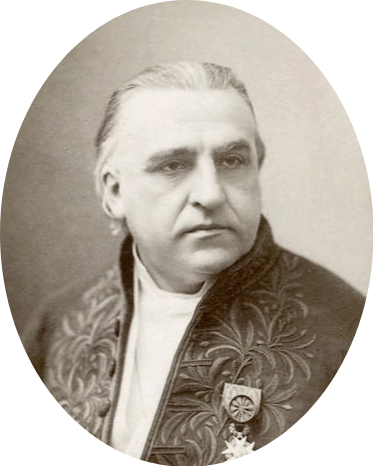
\includegraphics[width=.2\textwidth]{pic/Jean-Martin_Charcot-modified.png}
        \caption{J.-M. Charcot (1825-1893) (\href{https://fr.wikipedia.org/wiki/Jean-Martin_Charcot\#/media/Fichier:Jean-Martin\_Charcot.jpg}{Wikipédia}).}
        \end{figure}
        \begin{itemize}
        \small
        \item Père de la neurologie moderne
        \item Impact sur son \og{}réseau\fg{} \\
         {\footnotesize $\quad$Freud, de la Tourette, Babinski$\dots$
         }
        \item hystérie, SLA, Parkinson$\dots$
        \item Fonds Charcot sur SorbonNum\footnote{\url{https://patrimoine.sorbonne-universite.fr}}
%        \item Corpus Charcot sur \textsc{OBVIE}\footnote{\url{https://obtic.huma-num.fr/obvie/charcot/?view=corpus}}
        \end{itemize}
    \end{columns}
    
%    \begin{exampleblock}{}
%\centering
%    \color{deepblue}{\textmd{\textcolor{purple}{Pister numériquement la circulation du discours médical de Charcot}}}
%\end{exampleblock}

    

\end{frame}

\section[Problématique]{Problématique}
\begin{frame}{Double objectif}
	        \begin{figure}
		\centering
		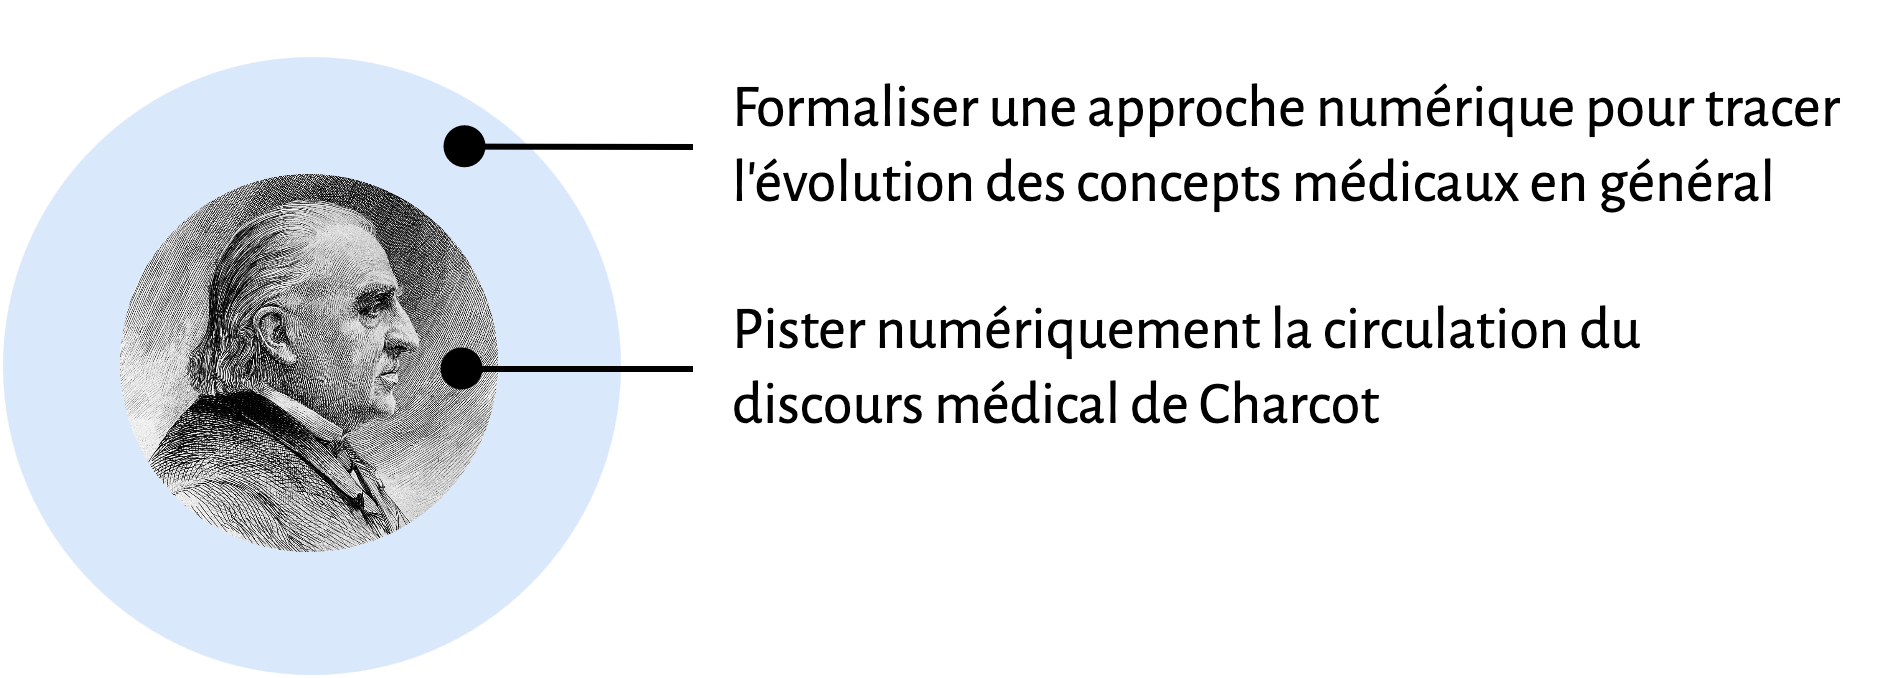
\includegraphics[width=1\textwidth]{pic/objectif_double2.png}
		%\caption{}
	\end{figure}

\begin{variableblock}{}{bg=white,fg=RubineRed}{bg=green,fg=red}
\centering
%Comment mesurer l'impact de Charcot sur son réseau scientifique ?
Quels sont les champs lexicaux dominants dans le discours de Charcot ?
\end{variableblock}

	
\end{frame}
\begin{frame}{Études numériques des circulations culturelles et scientifiques}
   \centering
    \resizebox{1\textwidth}{!}{ % Adjust the 0.8 value to scale the diagram as desired
    \begin{tikzpicture}[
        node distance=1.5cm and 1.5cm,
        box/.style={draw, rounded corners, fill=white, align=center, text width=3.5cm, font=\small, inner sep=5pt},
        central/.style={draw, rounded corners, fill=yellow!70, text width=2.5cm, font=\large\bfseries, align=center, inner sep=5pt},
        medical/.style={draw, rounded corners, fill=violet!30, text width=3.5cm, font=\small, align=center, inner sep=5pt},
        science/.style={draw, rounded corners, fill=blue!60, text width=3.5cm, font=\small, align=center, inner sep=5pt},
        label/.style={font=\small\bfseries, fill=magenta!80, text=white, rounded corners, inner sep=3pt, align=center, text width=4cm},
        edge from parent/.style={draw, thick, -{Stealth}}
    ]

    % Top label
    \node[label] at (0, 5) {Humanités numériques};

    % Boxes in the top row
    \node[box] (images) at (-4, 3) {Images \\ \textit{Visual Contagions} \\ (\cite{joyeux2019visual})};
    \node[box] (scientific) [below=of images] {Pensée scientifique \\ \textit{Claude Bernard} \\ (\cite{riguet2018impact})};
    \node[box] (allusions) [below=of scientific] {Allusions textuelles \\ (\cite{manjavacas})};
    
    \node[box] (manuscripts) at (4, 3) {Manuscrits \\ \textit{Katabase} \\ (\cite{gabay2021katabase})};
    \node[box] (entities) [below=of manuscripts] {Impact des entités, \\ \textit{Rankingdom} \\ (\cite{soulet2024})};
    \node[box, text width=4cm, xshift=0.3cm] (reuse) [below=of entities] {Réemplois textuels \\ \textit{ModERN} \\ (\cite{fedchenko2024recherche})};
    
    % Central "Circulations" node
    \node[central] (circulations) at (0, 0) {Circulations};

    % Medical discourse box - moved slightly lower with yshift
    \node[medical] (medical) [below=of circulations, yshift=-0.4cm] {Discours médical \\ (\cite{petkovic2023circulation})};

    % Bottom label and science history box
    \node[label, fill=blue!80, text width=4cm, anchor=north east] at (-6, -6) {Histoire des sciences};
    \node[science, below=of medical, fill=white, yshift=-0.3cm] (science) {\cite{broussolle2012} \\ \cite{tasca2012women} \\ \cite{bogousslavsky2020} \\ \cite{teive2022thomas} \\ \cite{camargo2024}};

    % Right label
    \node[label, fill=blue!80, text width=3cm, anchor=north west] at (6, -6) {Impact de Charcot};

    % Edges to central node
    \draw[edge from parent] (images) -- (circulations);
    \draw[edge from parent] (scientific) -- (circulations);
    \draw[edge from parent] (allusions) -- (circulations);
    \draw[edge from parent] (manuscripts) -- (circulations);
    \draw[edge from parent] (entities) -- (circulations);
    \draw[edge from parent] (reuse) -- (circulations);

    % Edge from circulations to medical discourse
    \draw[edge from parent] (circulations) -- (medical);
    \draw[edge from parent] (medical) -- (science);

    \end{tikzpicture}
    } % End of resizebox
%\begin{figure}[!h]
%		\centering
%		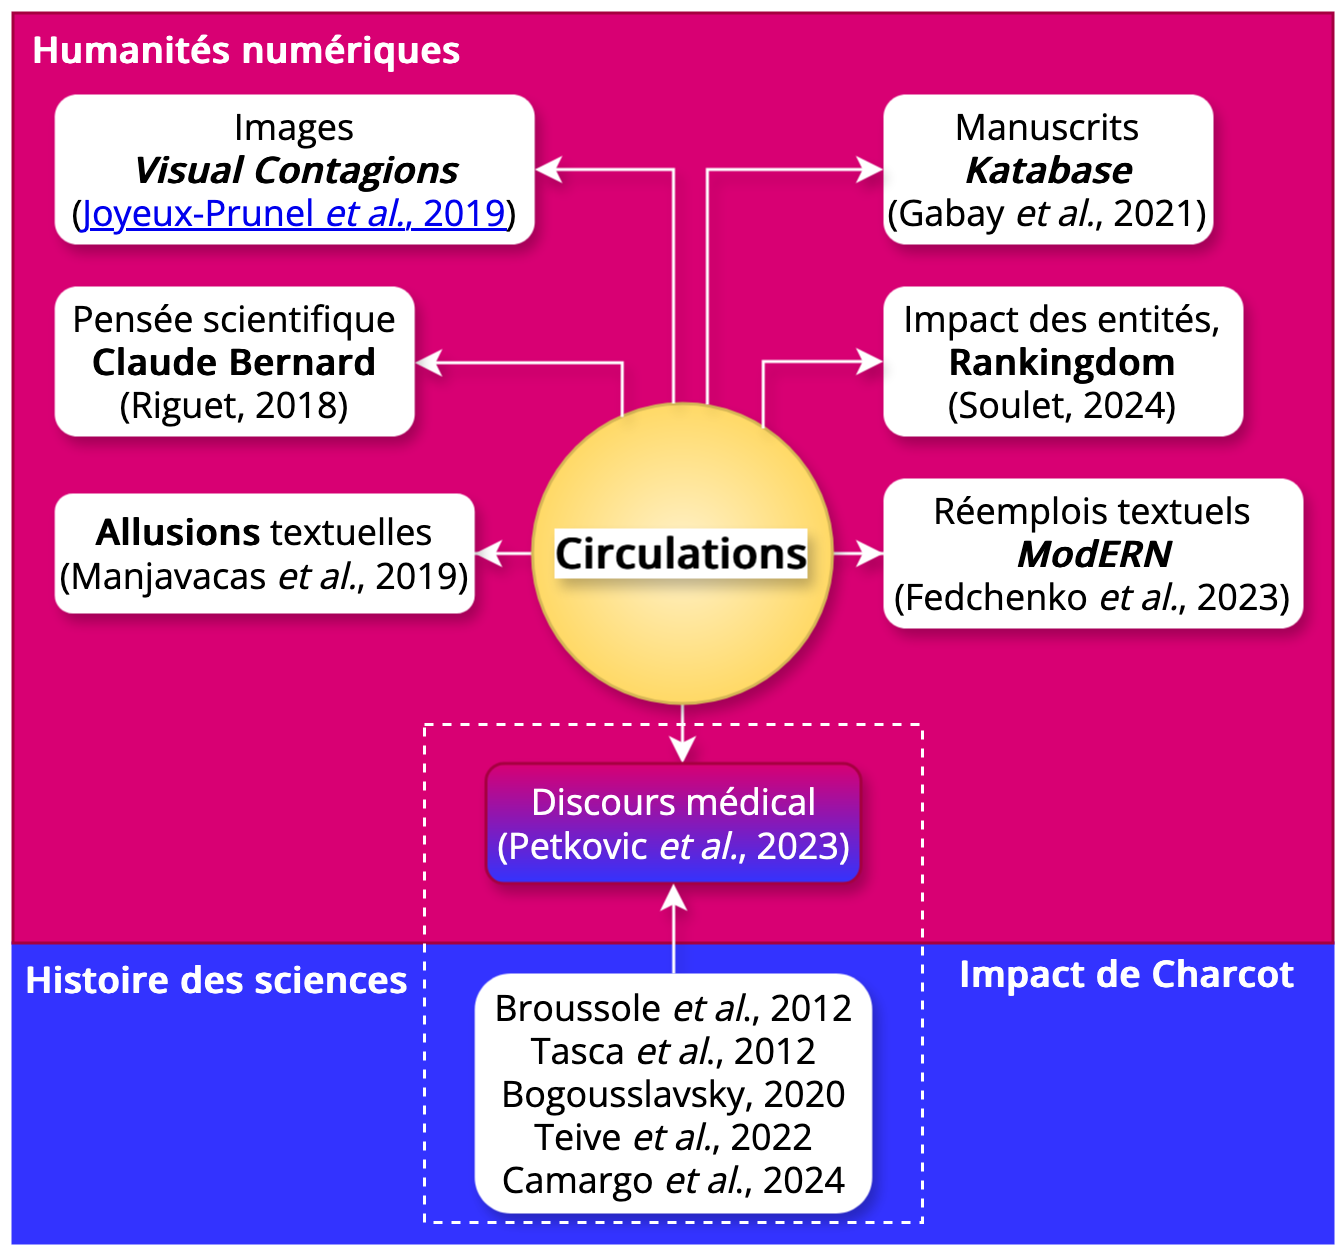
\includegraphics[width=0.7\textwidth]{pic/test.png}
%		\caption{Analyse de quadrant : positionnement de l'entité \texttt{Charcot} au sein de son domaine.}
%	\end{figure}
%	\begin{itemize}
%	\item réception de la pensée scientifique de C. Bernard \citep{riguet2018impact}
%	\item détection des réemplois textuels
%\citep{fedchenko2024recherche}
%	\item Rankingdom -- mesurer l'importance d’une entité \citep{soulet2024}
%	\end{itemize}
%		        \begin{figure}[!h]
%		\centering
%		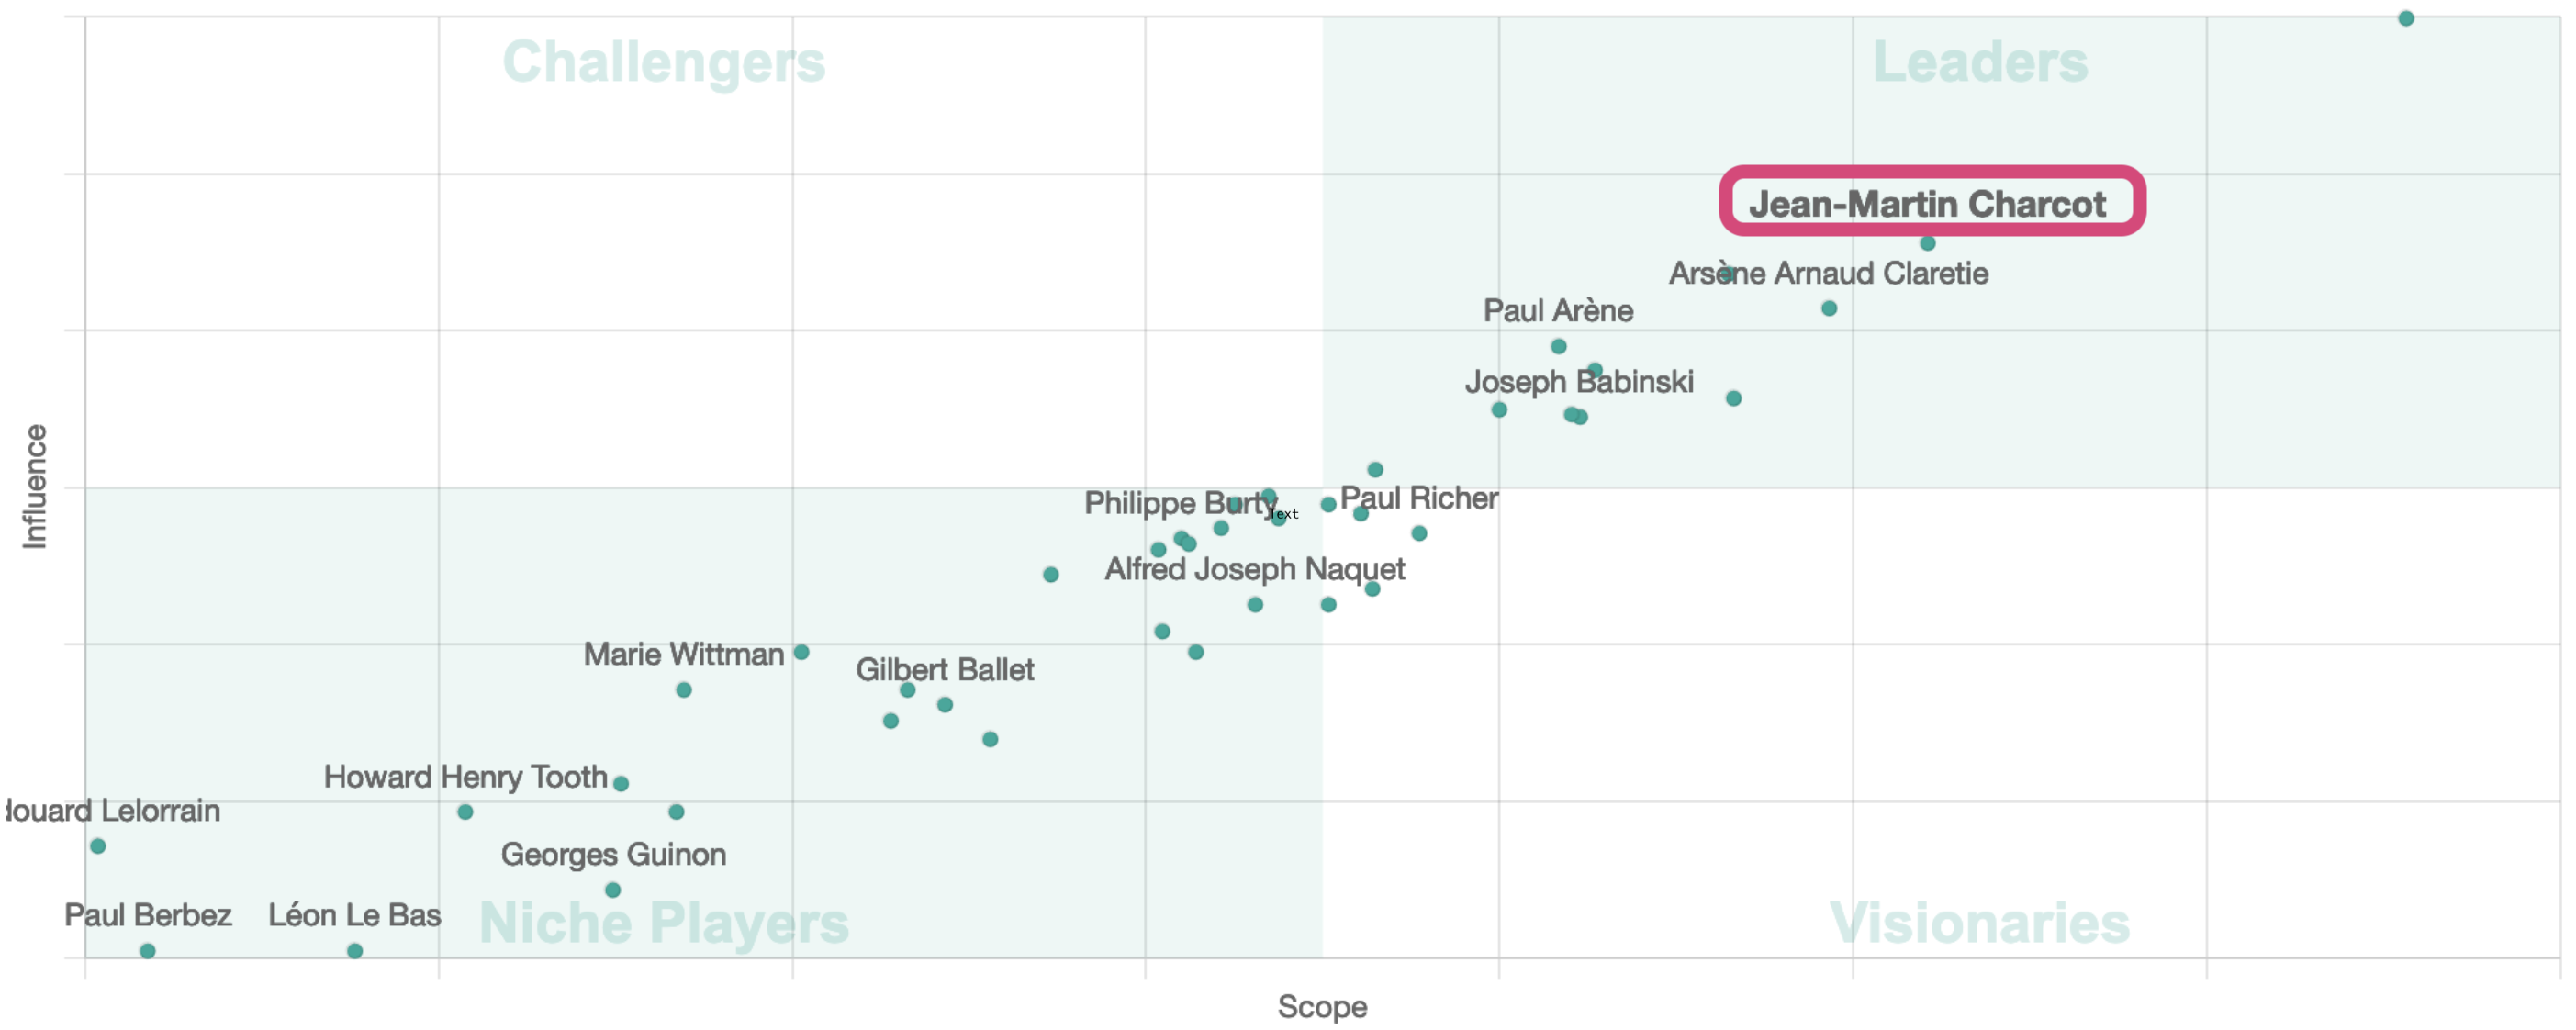
\includegraphics[width=0.8\textwidth]{pic/analyse_quadrant2.png}
%		\caption{Positionnement de l'entité \texttt{Charcot} au sein de son domaine \textit{via} l'analyse de quadrant.}
%	\end{figure}
\end{frame}

\begin{frame}{Analyse de l'impact de l'entité \texttt{Charcot} \textit{via} Rankingdom}
\begin{figure}[!h]
		\centering
		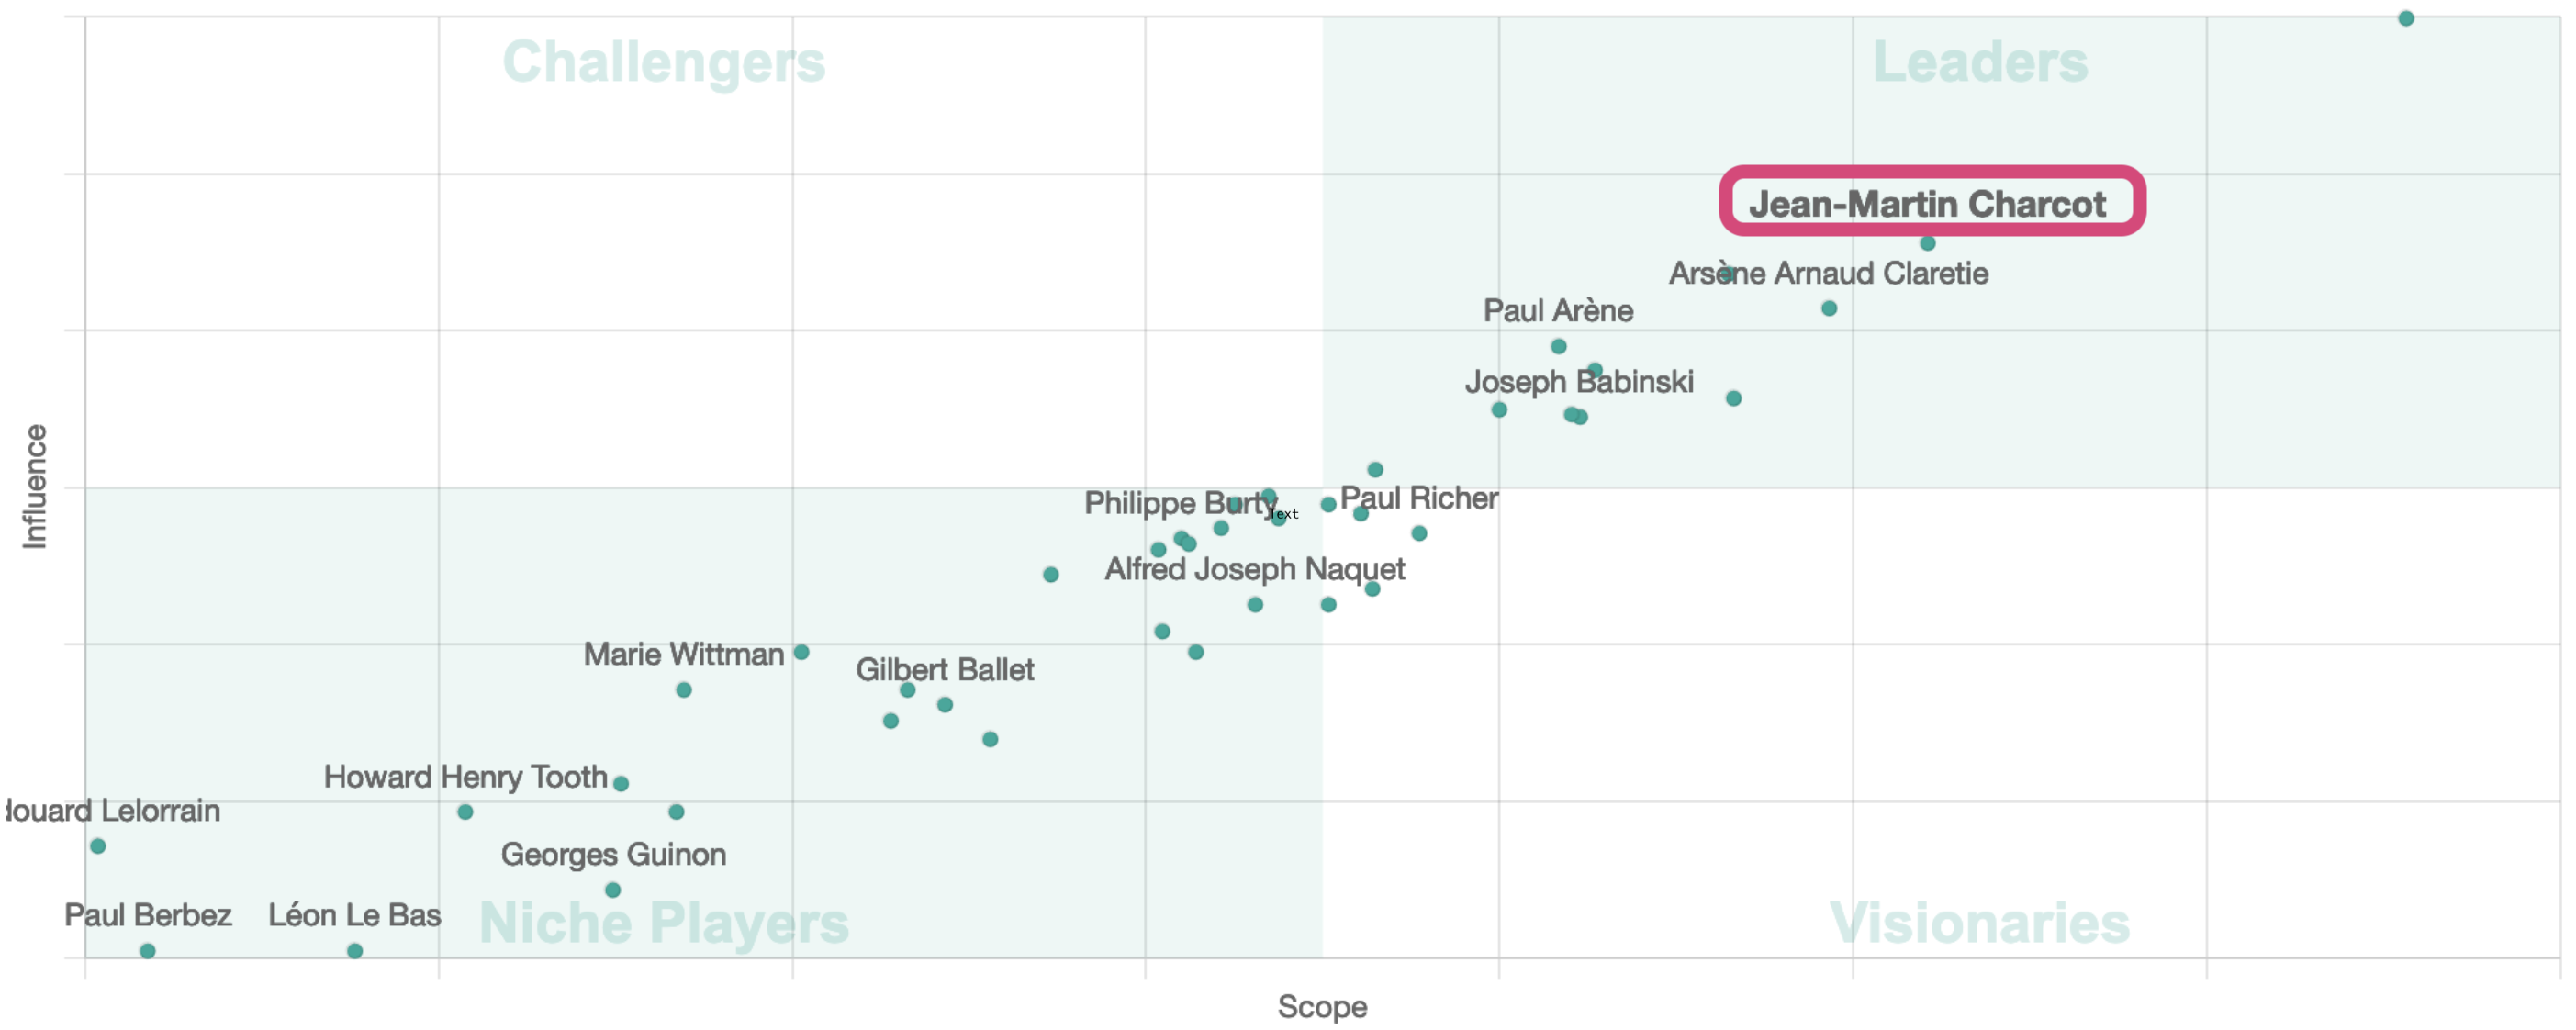
\includegraphics[width=0.7\textwidth]{pic/analyse_quadrant2.png}
		\caption{Analyse de quadrant : positionnement de l'entité \texttt{Charcot} au sein de son domaine.}
		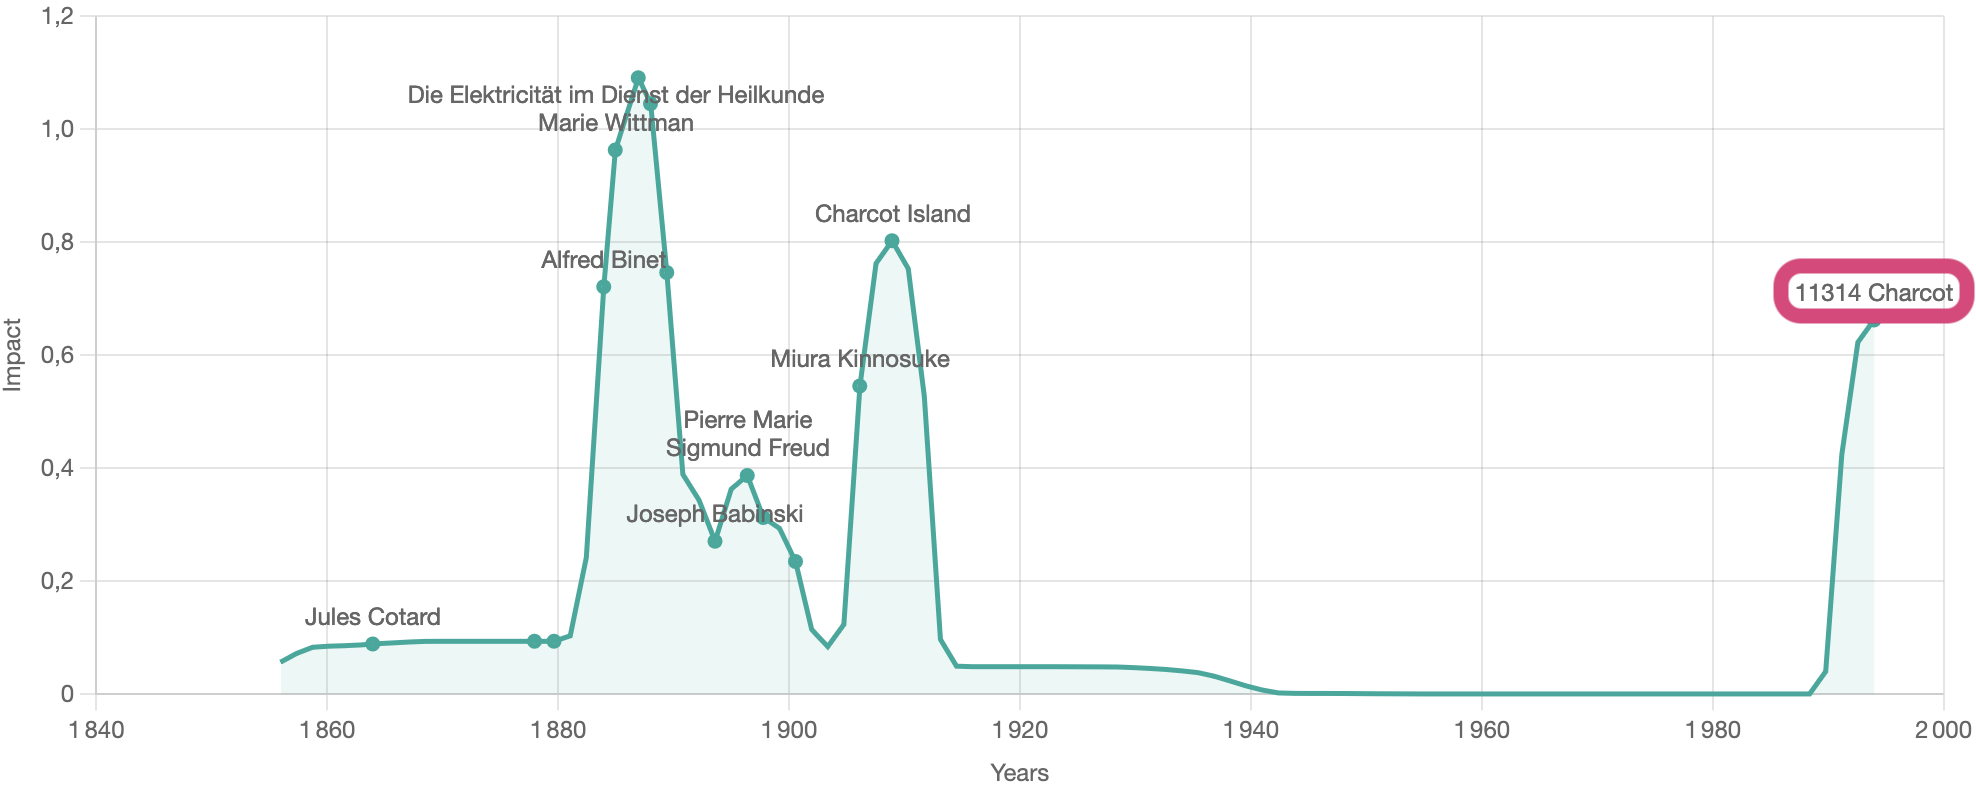
\includegraphics[width=0.7\textwidth]{pic/impact_temporel.png}
		\caption{Analyse temporelle de l'impact de l'entité \texttt{Charcot}.}
	\end{figure}
\end{frame}


\section[Méthodologie]{Méthodologie}
\begin{frame}{Mesurer le degré d'intertextualité}
Mesurer informatiquement l'impact de Charcot sur son \og{}réseau\fg{} \\$\rightarrow$ intertextualité uni-directionnelle\\
\begin{itemize}
\item {\small rapports entre une œuvre et d'autres qui l'ont précédée ou suivie \\
\begin{flushright} 
(\cite{riffaterre1980trace})}
\end{flushright}
\end{itemize}
\begin{figure}[!h]
    \centering
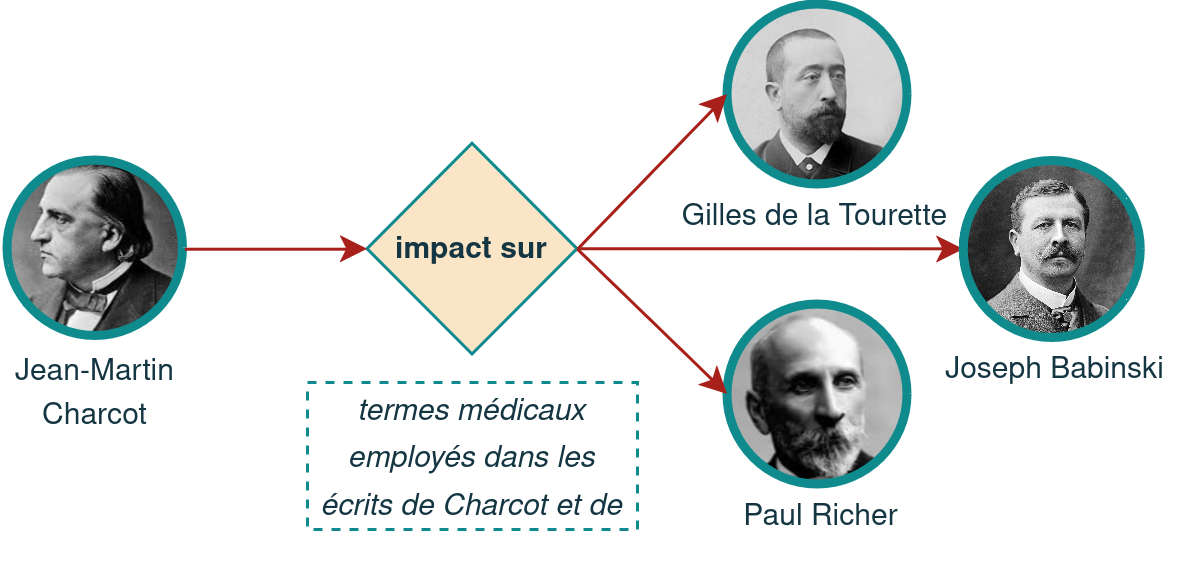
\includegraphics[width=100mm,scale=0.5]{pic/charcot_intertextualite.png}
    \caption{Opérationnalisation de l'impact de Charcot sur ses élèves.}
    \label{fig:my_label}
\end{figure}
\end{frame}

\begin{frame}{Corpus Charcot}
\begin{block}{SorbonNum\footnote{\tiny{\url{https://patrimoine.sorbonne-universite.fr/}}} | Bibliothèque de Sorbonne Université (BSU)}
201 documents XML OCRisés (sans post-correction)
\end{block}
\begin{itemize}
    \item \textrm{Charcot} : textes rédigés par Charcot
    \item \textrm{Autres} : textes rédigés par son réseau scientifique
\end{itemize}
\begin{table}[!ht]
    \centering
    \begin{tabular}{|c|c|c|}
    \hline 
    \rowcolor{gray!30}
       Corpus & Nb de docs & Nb de tokens \\
       \hline
       \textrm{Charcot}  & 68 & 12 190 649 (38,12 \%) \\
       \textrm{Autres}  & 133 & 19 788 830 (61,88 \%) \\
       \hline\hline
       \textbf{Total} & \textbf{201} & \textbf{31 979 479} (100 \%)\\
       \hline
    \end{tabular}
    \caption{Répartition du corpus issu du fonds Charcot\footnote{\tiny{\url{https://patrimoine.sorbonne-universite.fr/collection/Fonds-Charcot}}}.}
    \label{tab:my_label}
\end{table}
\end{frame}

\begin{frame}{OBVIE -- recherche textuelle, corpus Charcot\footnote{\url{https://obtic.huma-num.fr/obvie/charcot/?view=corpus}}}
\textsc{OBVIE} : moteur de recherche avancée {\small\citep{alrahabi2022obvie}}\\
{\small \danger quantification de l'importance des \og{}collocations\fg{} (\cite{nerima2006})}
\begin{figure}[!h]
    \centering
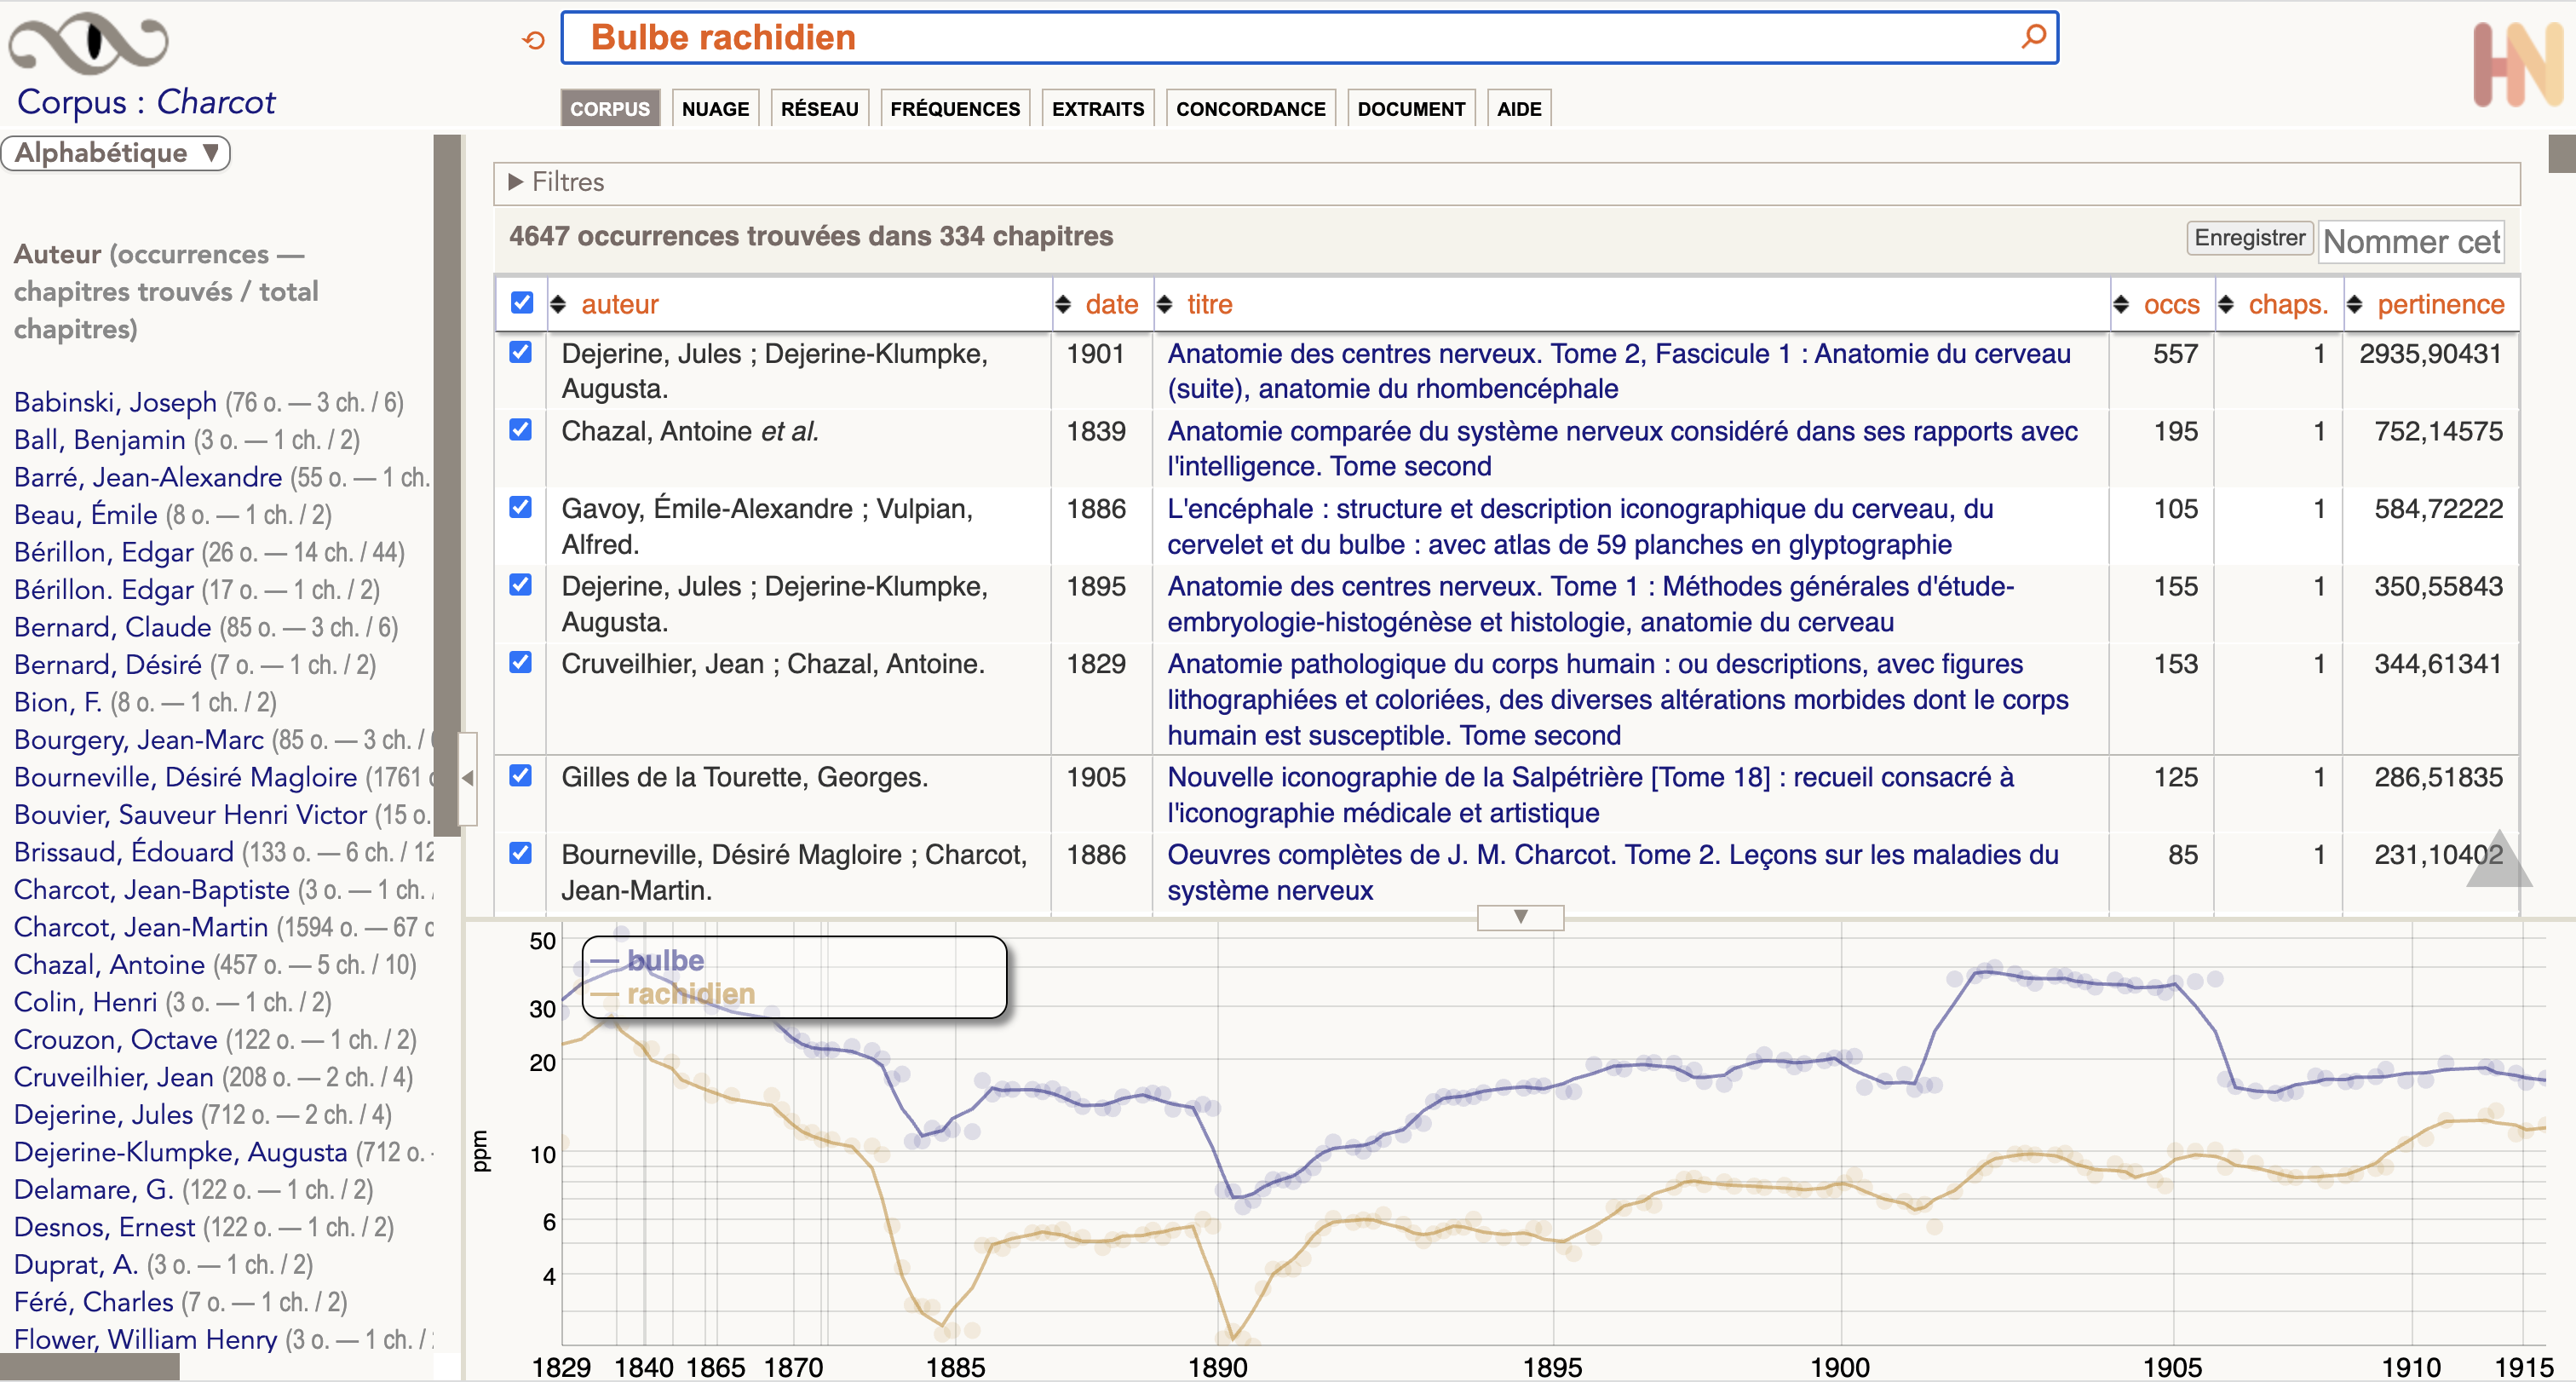
\includegraphics[width=90mm,scale=0.5]{pic/bulbe_rachidien_mini.png}
    \caption{Distribution des fréquences des tokens avec la frise chronologique pour ceux constituant l'expression \textit{bulbe rachidien} (issus des corpus \og{}Charcot\fg{} et \og{}Autres\fg{}).}
    \label{fig:my_label}
\end{figure}
% citations directes (\cite{manjavacas2019})
\end{frame}

\begin{frame}{OBVIE -- comparaison des documents similaires}
\begin{itemize}
\item fouille avancée des corpus en \textsc{XML-TEI}
\item textes similaires : mots fréquents / en commun, noms cités
\end{itemize}
%\danger impossible de quantifier l'importance des MWEs
\begin{figure}[!h]
    \centering
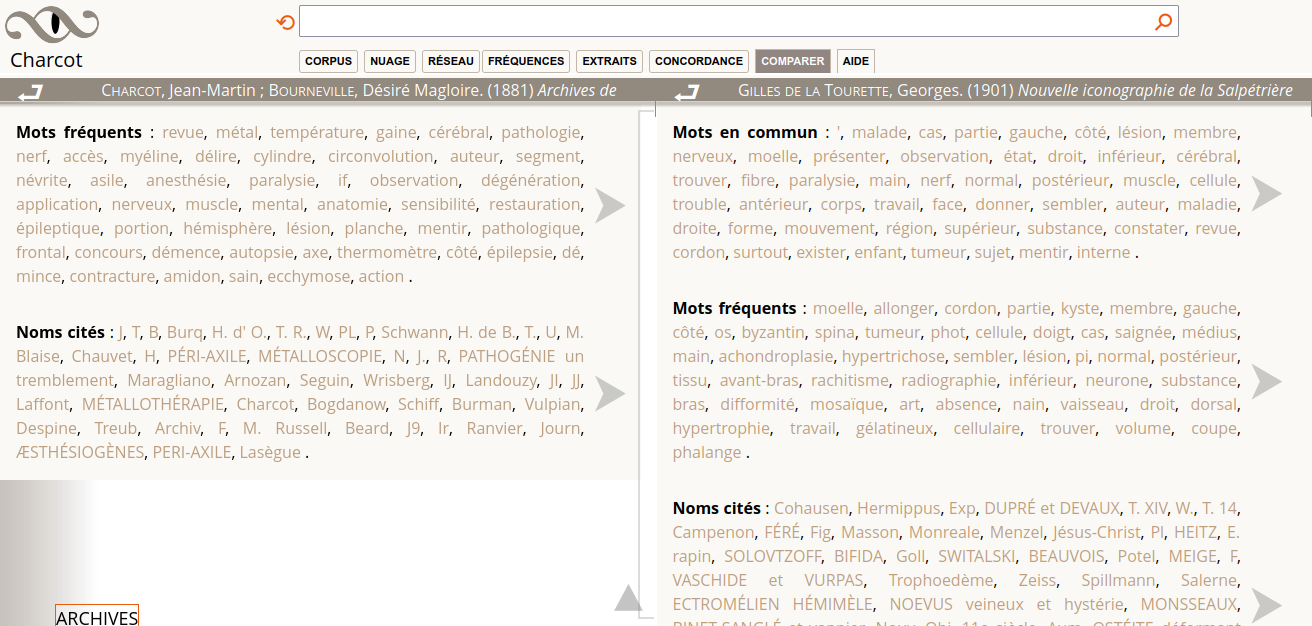
\includegraphics[width=100mm,scale=0.5]{pic/doc_sim.png}
    \caption{Points similaires entre un ouvrage de Charcot et celui de de la Tourette.}
%    \caption{Distribution des fréquences des tokens avec la frise chronologique pour ceux constituant l'expression \textit{bulbe rachidien} (issus des corpus \og{}Charcot\fg{} et \og{}Autres\fg{}).}
    \label{fig:my_label}
\end{figure}
% citations directes (\cite{manjavacas2019})
\end{frame}

\begin{frame}{TextPair -- alignement de textes, corpus Charcot\footnote{\url{https://anomander.uchicago.edu/text-pair/charcot2autres/}}}
\danger nombre de
résultats assez conséquent -- filtrage nécessaire
    \begin{figure}[!ht]
        \centering
        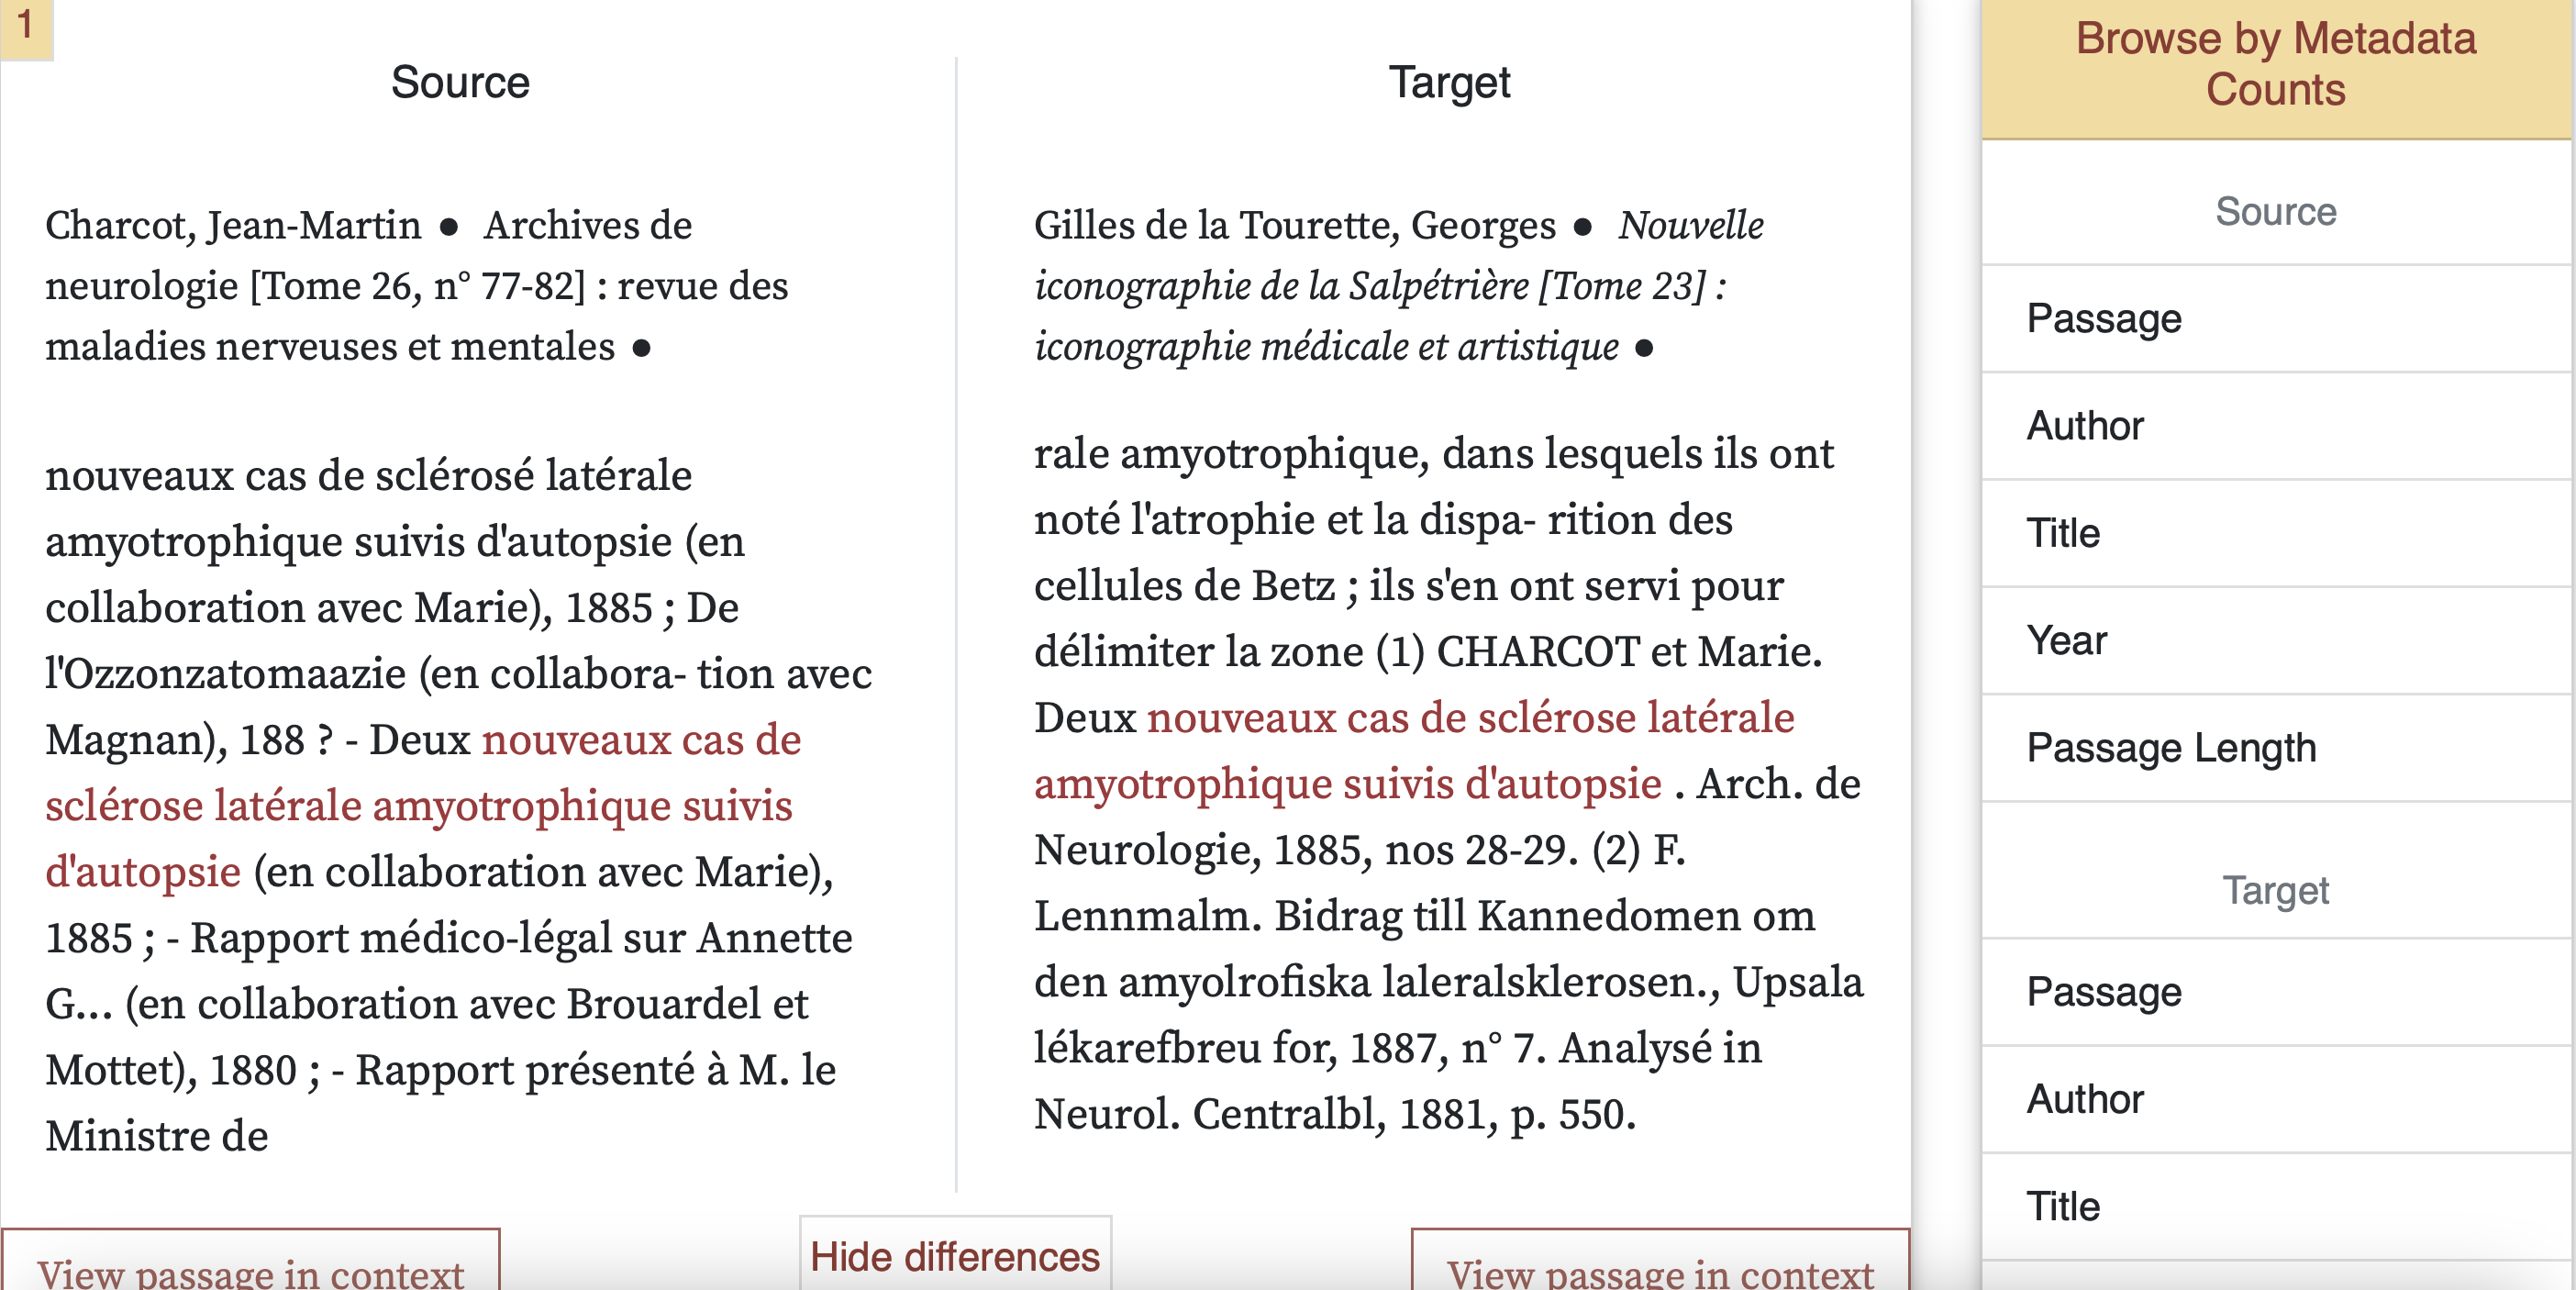
\includegraphics[width=90mm,scale=0.5]{pic/textpair.png}
        \caption{Alignement et comparaison des textes de
Charcot à celui de Georges Gilles de la Tourette (le seul
résultat) en lançant la requête \textit{sclérose latérale
amyotrophique}.}
        \label{fig:enter-label}
    \end{figure}
\end{frame}



\begin{frame}{Liste des concepts médicaux}
Extraction semi-automatique des termes en lien avec Charcot.\\~\\

 \begin{figure}[!htb]
    \centering
    \begin{minipage}{.5\textwidth}
        \centering
        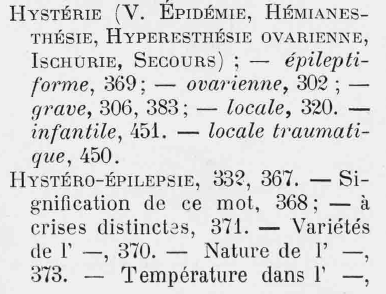
\includegraphics[width=0.6\linewidth, height=0.3\textheight]{pic/concepts-pdf}
        \caption{Index des termes \citep{charcot1890oeuvres}.}
        \label{fig:prob1_6_2}
    \end{minipage}%
    \begin{minipage}{.5\textwidth}
        \centering
        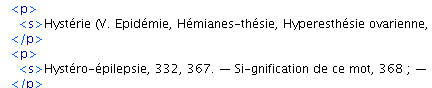
\includegraphics[width=1\linewidth, height=0.15\textheight]{pic/concepts-xml}
        \caption{Concepts médicaux, document XML.}
        \label{fig:prob1_6_1}
    \end{minipage}
\end{figure}
\begin{figure}[!htb]
    \centering
    \begin{minipage}{.5\textwidth}
        \centering
        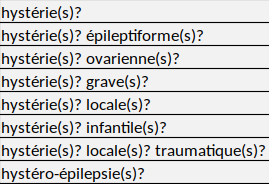
\includegraphics[width=0.6\linewidth, height=0.25\textheight]{pic/concepts-csv}
        \caption{Liste finale des concepts médicaux.}
        \label{fig:prob1_6_2}
    \end{minipage}%
    \begin{minipage}{.6\textwidth}
        \centering
   \begin{enumerate}
   \setcounter{enumi}{3}
   \item entre \texttt{<s>} et \texttt{,-(} (regex)
   \item sans termes génériques (\textit{os}, \textit{peau})
\item prise en compte des sg. / pl. (regex)
   \end{enumerate}
    \end{minipage}
\end{figure}
\end{frame}




\section[Résultats]{Résultats}
%\begin{frame}{Extraction des phrases-clés $\cdot$ méthode supervisée}
		        \begin{figure}[!h]
		\centering
		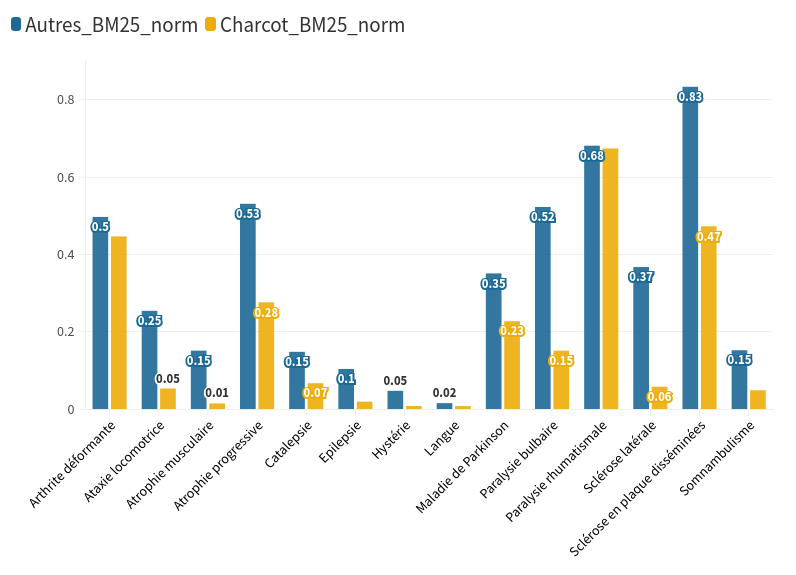
\includegraphics[width=0.6\textwidth]{pic/Charcot_Autres_250523.png}
		\caption{Visualisation de pertinence des concepts dans les deux corpus suivant la métrique \textsc{BM25} \citep{robertson1976relevance}.}
	\end{figure}
	\textsc{BERT} \citep{vaswani2023} : diplopie, myélite partielle$\dots$ (Charcot)\\
	\quad\quad\quad vicieuses, délire, miracle$\dots$ (Autres)
\end{frame}
%\begin{frame}{Extraction des phrases-clés $\cdot$ méthode non-supervisée}
		        \begin{figure}[!h]
		\centering
		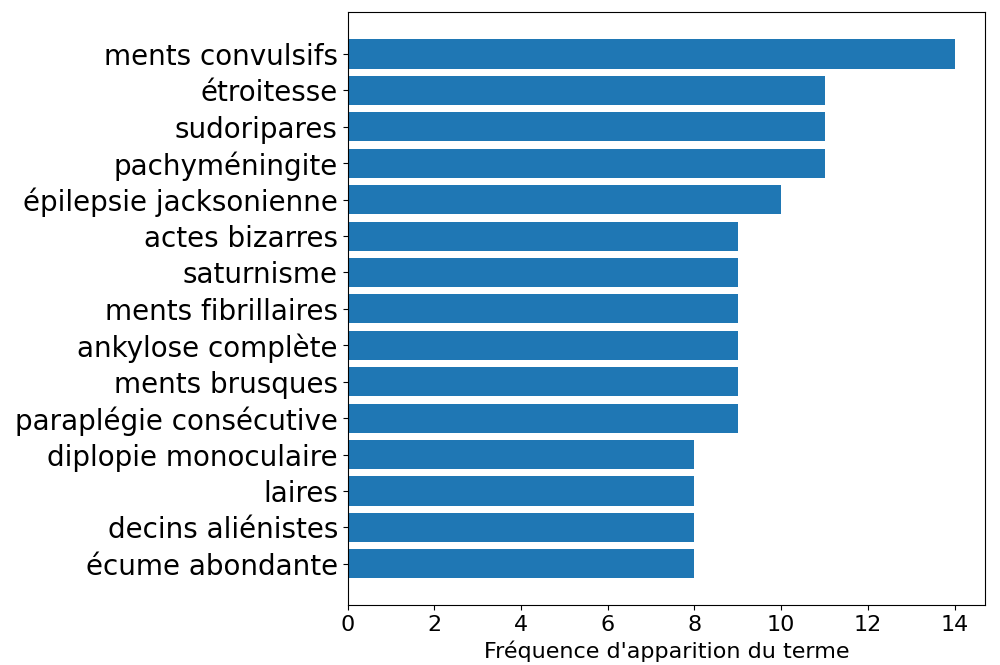
\includegraphics[width=0.8\textwidth]{pic/termes_partages.png}
		\caption{Les 15 termes les plus fréquents partagés par Charcot et son réseau selon \texttt{keyphrase-vectorizers}\footnote{\url{https://pypi.org/project/keyphrase-vectorizers/}}.}
	\end{figure}
\end{frame}
\begin{frame}{Calcul de pertinence des concepts}
Trois mesures de pondération : \textsc{TF-IDF}, \textsc{BM25} et \textsc{BERT}.
    \footnotesize
\begin{table}[]
\begin{tabular}{|l|cccc|}
\hline
\multicolumn{1}{|c|}{\multirow{}{}{Terme}} & \multicolumn{4}{c|}{\cellcolor{gray!10!white}{ Corpus \textrm{Autres}}}                              \\ \cline{2-5} 
\multicolumn{1}{|c|}{}                       & \multicolumn{1}{c}{{Fréquence}} & \multicolumn{1}{c}{{TF-IDF}} & \multicolumn{1}{c}{{BM25}}  & {BERT} \\ \hline
{Arthrite déformante} &
  \multicolumn{1}{|r|}{{24}} &
  \multicolumn{1}{|r|}{{0,02}} &
  \multicolumn{1}{|r|}{{0,50}} &
  {0,40} \\ \hline
{Ataxie locomotrice} &
  \multicolumn{1}{|r|}{{169}} &
  \multicolumn{1}{|r|}{{0,08}} &
  \multicolumn{1}{|r|}{{0,25}} &
  {0,39} \\ \hline
{Atrophie musculaire} &
  \multicolumn{1}{|r|}{{1465}} &
  \multicolumn{1}{|r|}{{0,43}} &
  \multicolumn{1}{|r|}{{0,15}} &
  {0,42} \\ \hline
{Atrophie progressive} &
  \multicolumn{1}{|r|}{{22}} &
  \multicolumn{1}{|r|}{{0,02}} &
  \multicolumn{1}{|r|}{{0,53}} &
  {0,39} \\ \hline
{Catalepsie} &
  \multicolumn{1}{|r|}{{975}} &
  \multicolumn{1}{|r|}{{0,28}} &
  \multicolumn{1}{|r|}{{0,15}} &
  {0,39} \\ \hline
{Épilepsie} &
  \multicolumn{1}{|r|}{{577}} &
  \multicolumn{1}{|r|}{{0,12}} &
  \multicolumn{1}{|r|}{{0,10}} &
  {0,41} \\ \hline
{Hystérie} &
  \multicolumn{1}{|r|}{{4934}} &
  \multicolumn{1}{|r|}{{0,45}} &
  \multicolumn{1}{|r|}{{0,05}} &
  {0,41} \\ \hline
{Langue} &
  \multicolumn{1}{|r|}{{3591}} &
  \multicolumn{1}{|r|}{{0,11}} &
  \multicolumn{1}{|r|}{{0,02}} &
  {0,41} \\ \hline
{Maladie de Parkinson} &
  \multicolumn{1}{|r|}{{130}} &
  \multicolumn{1}{|r|}{{0,09}} &
  \multicolumn{1}{|r|}{{0,35}} &
  {0,37} \\ \hline
{Paralysie bulbaire} &
  \multicolumn{1}{|r|}{{93}} &
  \multicolumn{1}{|r|}{{0,09}} &
  \multicolumn{1}{|r|}{{0,52}} &
  {0,40} \\ \hline
{Paralysie rhumatismale} &
  \multicolumn{1}{|r|}{{14}} &
  \multicolumn{1}{|r|}{{0,02}} &
  \multicolumn{1}{|r|}{{0,68}} &
  {\cellcolor{green!30!white}{\textcolor{purple}{\textbf{0,44}}}} \\ \hline
{Sclérose latérale} &
  \multicolumn{1}{|r|}{{127}} &
  \multicolumn{1}{|r|}{{0,09}} &
  \multicolumn{1}{|r|}{{0,37}} &
  {0,41} \\ \hline
{Sclérose en plaque disséminées} &
  \multicolumn{1}{|r|}{{12}} &
  \multicolumn{1}{|r|}{{0,02}} &
  \multicolumn{1}{|r|}{\cellcolor{green!30!white}{\textcolor{purple}{\textbf{0,83}}}} &
  {0,40} \\ \hline
{Somnambulisme} &
  \multicolumn{1}{|r|}{{3410}} &
  \multicolumn{1}{|r|}{\cellcolor{green!30!white}{\textcolor{purple}{\textbf{1}}}} &
  \multicolumn{1}{|r|}{{0,15}} &
  {0,43} \\ \hline
\end{tabular}
\caption{Pertinence des concepts sous forme des scores TF-IDF, BM25 et BERT, corpus \textrm{Autres}.}
\end{table}
\end{frame} 

\begin{frame}{Intensification du discours
de Charcot dans le corpus \textrm{Autres}}
Le terme le plus impactant dans le réseau de Charcot selon \textsc{BM25} :\\
\textit{sclérose en plaque disséminées} ? (pertinence : 83\%)
\begin{figure}[!h]
    \centering
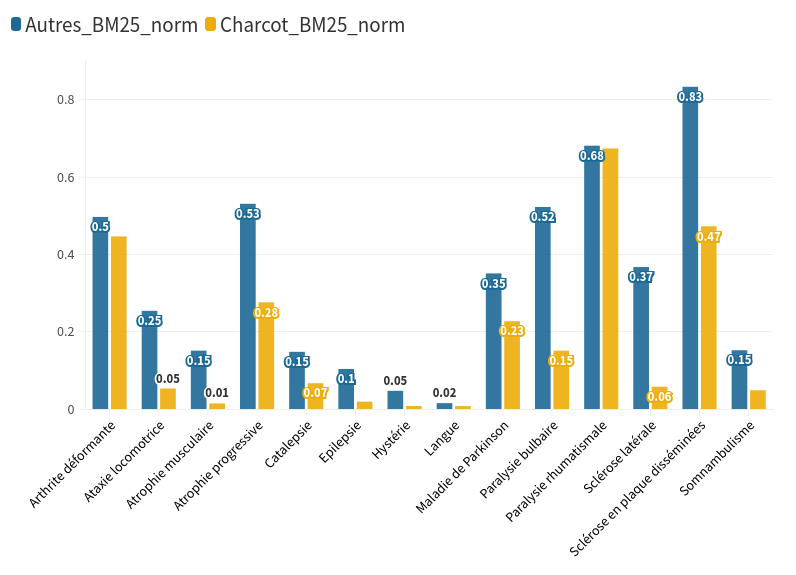
\includegraphics[width=80mm,scale=0.5]{pic/Charcot_Autres_250523.png}
    \caption{Pertinence des concepts dans les deux corpus (BM25).}
    \label{fig:my_label}
\end{figure}
\end{frame}

\begin{frame}{Types de concepts extraits avec \textsc{BERT}}
    \begin{itemize}
        \item plongements lexicaux et des
mécanismes d’attention
        \item modèle \texttt{bert-base-multilingual-cased}
    \end{itemize}
    \begin{flushright}
    {(\small \cite{vaswani2017})}
    \end{flushright}

\begin{table}[]
\begin{tabular}{|ll|ll|}
\hline
\multicolumn{2}{|c|}{\cellcolor[HTML]{EFEFEF}Corpus \textrm{Charcot}} & \multicolumn{2}{c|}{\cellcolor[HTML]{EFEFEF}Corpus \textrm{Autres}}     \\ \hline
\multicolumn{1}{|l|}{diplopie}                & 0,92 & \multicolumn{1}{l|}{préambule}       & 0,47      \\
\multicolumn{1}{|l|}{myélite partielle}       & 0,91 & \multicolumn{1}{l|}{délire}          & 0,47      \\
\multicolumn{1}{|l|}{état de mal épileptique} & 0,91 & \multicolumn{1}{l|}{miracle}         & 0,47      \\
\multicolumn{1}{|l|}{paralysie labio-glosso-laryngée} & 0,91 & \multicolumn{1}{l|}{cicatrices vicieuses} & 0,46 \\ \hline
\multicolumn{2}{|c|}{\cellcolor[HTML]{E1FFE1}\textsc{pathologies}}     & \multicolumn{2}{c|}{\cellcolor[HTML]{FFDFDD}\textsc{notions abstraites}} \\ \hline 
\end{tabular}
\end{table}
\end{frame}

\begin{frame}{Extraction des phrases-clés : méthode \texttt{keybert}}
\begin{enumerate}
\small
\item entrée : un document
\item tokénisation du document en phrases-clés candidates (PCC)
\item génération des plongements du doc. et des PCC par un modèle de langage
\item calcul de la similarité cosinus entre le document et les PC
\end{enumerate}
\begin{figure}
    \centering
    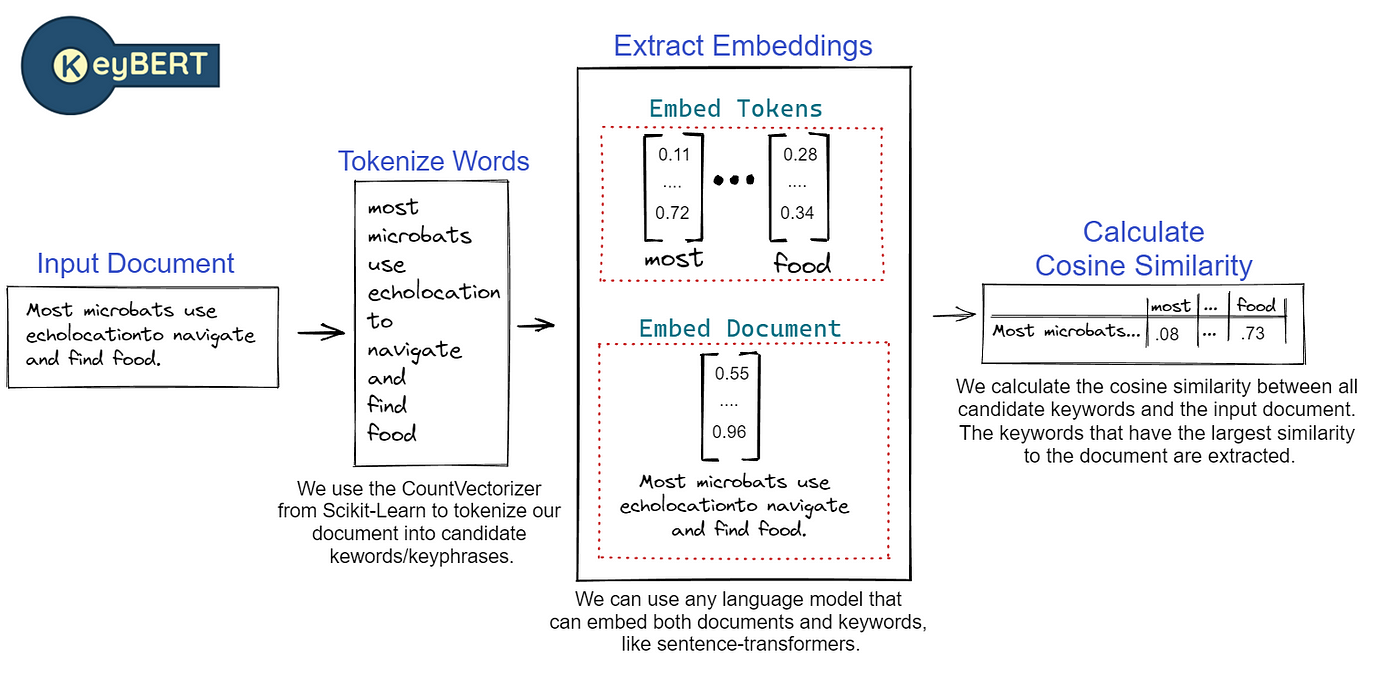
\includegraphics[width=80mm,scale=0.5]{pic/keybert.png}
    \caption{\textit{Pipeline} de la librairie \texttt{keybert} \citep{grootendorst2020keybert}.}
    \label{fig:enter-label}
\end{figure}
\end{frame}

\begin{frame}{Limitations de \texttt{keybert}}
\danger{} manque de diversification des résultats + (non-)grammaticalité\\
{\small 2 termes communs : \og{}articulations de épaule\fg{}, \og{}paralysie faciale périphérique\fg{}}
    \begin{figure}[!ht]
        \centering
        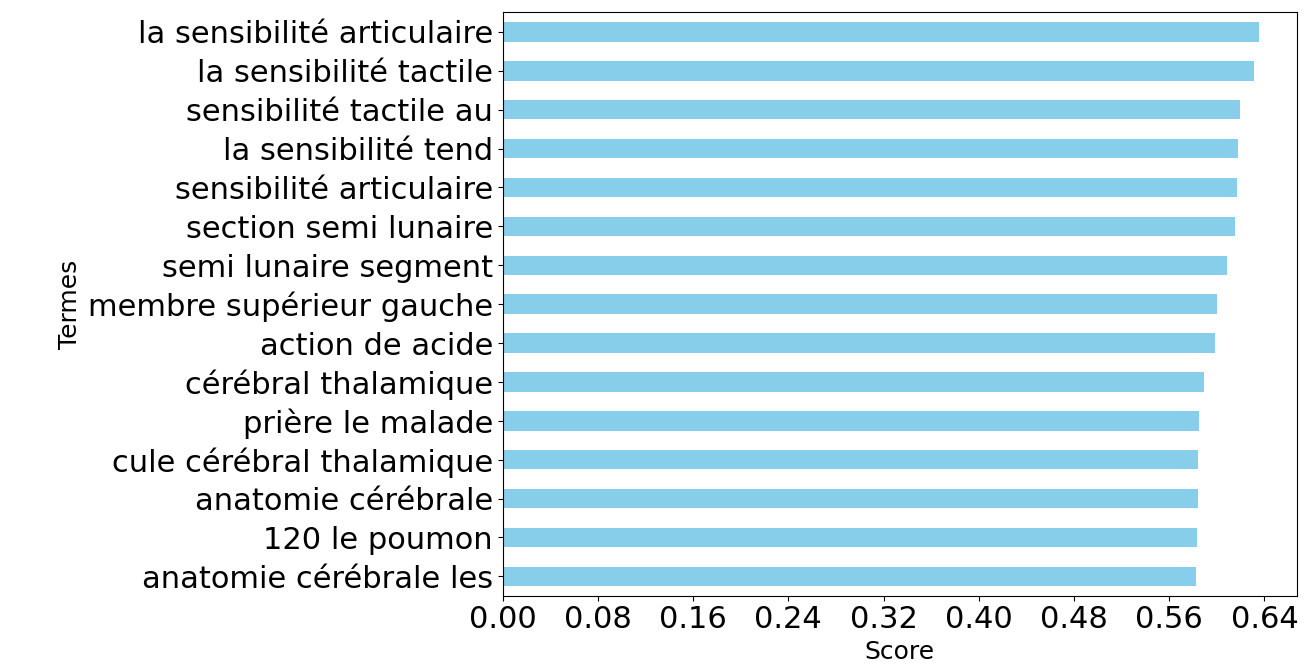
\includegraphics[width=100mm,scale=0.5]{pic/termes_keybert_autres.png}
        \caption{Répartition des 15 termes les plus pertinents dans le corpus \textrm{Autres} selon \texttt{keybert}.}
        \label{fig:enter-label}
    \end{figure}
\end{frame}

%\begin{frame}{Phrases-clés \textit{hapax} partagés dans les deux corpus selon \texttt{keybert}}
%Les seuls termes partagés avec le corpus Charcot : 
%%\begin{itemize}
%%\item articulations de [\textit{sic}] épaule
%%\item paralysie faciale périphérique
%%\end{itemize}
%    \begin{figure}[!ht]
%        \centering
%        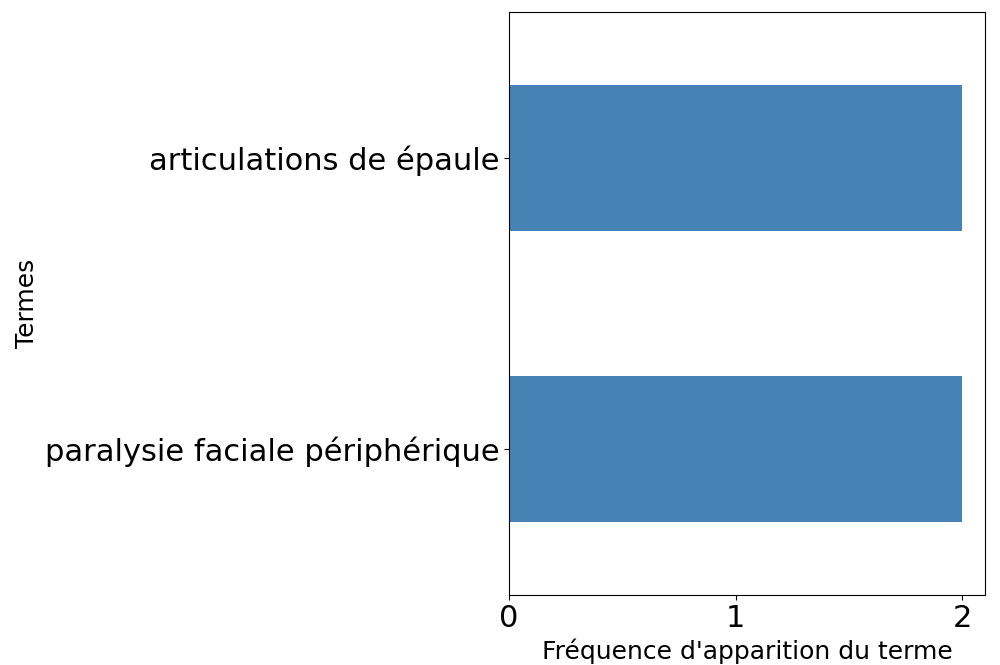
\includegraphics[width=90mm,scale=0.5]{pic/termes_partages_keybert.png}
%        \caption{Répartition des termes les plus pertinents dans les deux corpus selon \texttt{keybert}.}
%        \label{fig:enter-label}
%    \end{figure}
%\end{frame}
\begin{frame}{Extraction des phrases-clés : méthode \textit{PatternRank}\\
\quad \quad \quad\ \quad \quad \quad \quad \quad \quad \quad \ \ \ \ \ \small{Librairie \texttt{keyphrase-vectorizers}}}
%\begin{itemize}
%\item extraction des phrases-clés non-supervisée
%\item exploite des modèles de langues pré-entraînés + parties du discours
%\end{itemize}
\begin{enumerate}
\small
\item entrée : un seul document texte tokenisé
\item étiquetage des tokens avec les balises du partie du discours (POS)
\item sélection des tokens selon le motif POS $\rightarrow$ phrases-clés candidates (PCC)
\item génération des plongements du doc. et des PCC par un modèle de langue
\item calcul des similarités cosinus entre ces deux types de plongements +  \\classement des PCC par ordre décroissant
\item extraction des \textit{N} PC les plus représentatives
\end{enumerate}
\begin{figure}
    \centering
    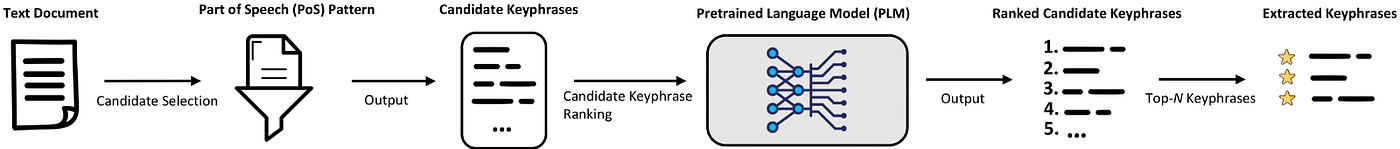
\includegraphics[width=110mm,scale=0.5]{pic/patternrank_workflow.png}
    \caption{\textit{Workflow} de la méthode \textit{PatternRank} \citep{schopf2022}.}
    \label{fig:enter-label}
\end{figure}
\notecite{schopf2022}
\end{frame}

%\begin{frame}{Termes partagés extraits avec \texttt{keyphrase-vectorizers}}
%    \begin{figure}[!ht]
%        \centering
%        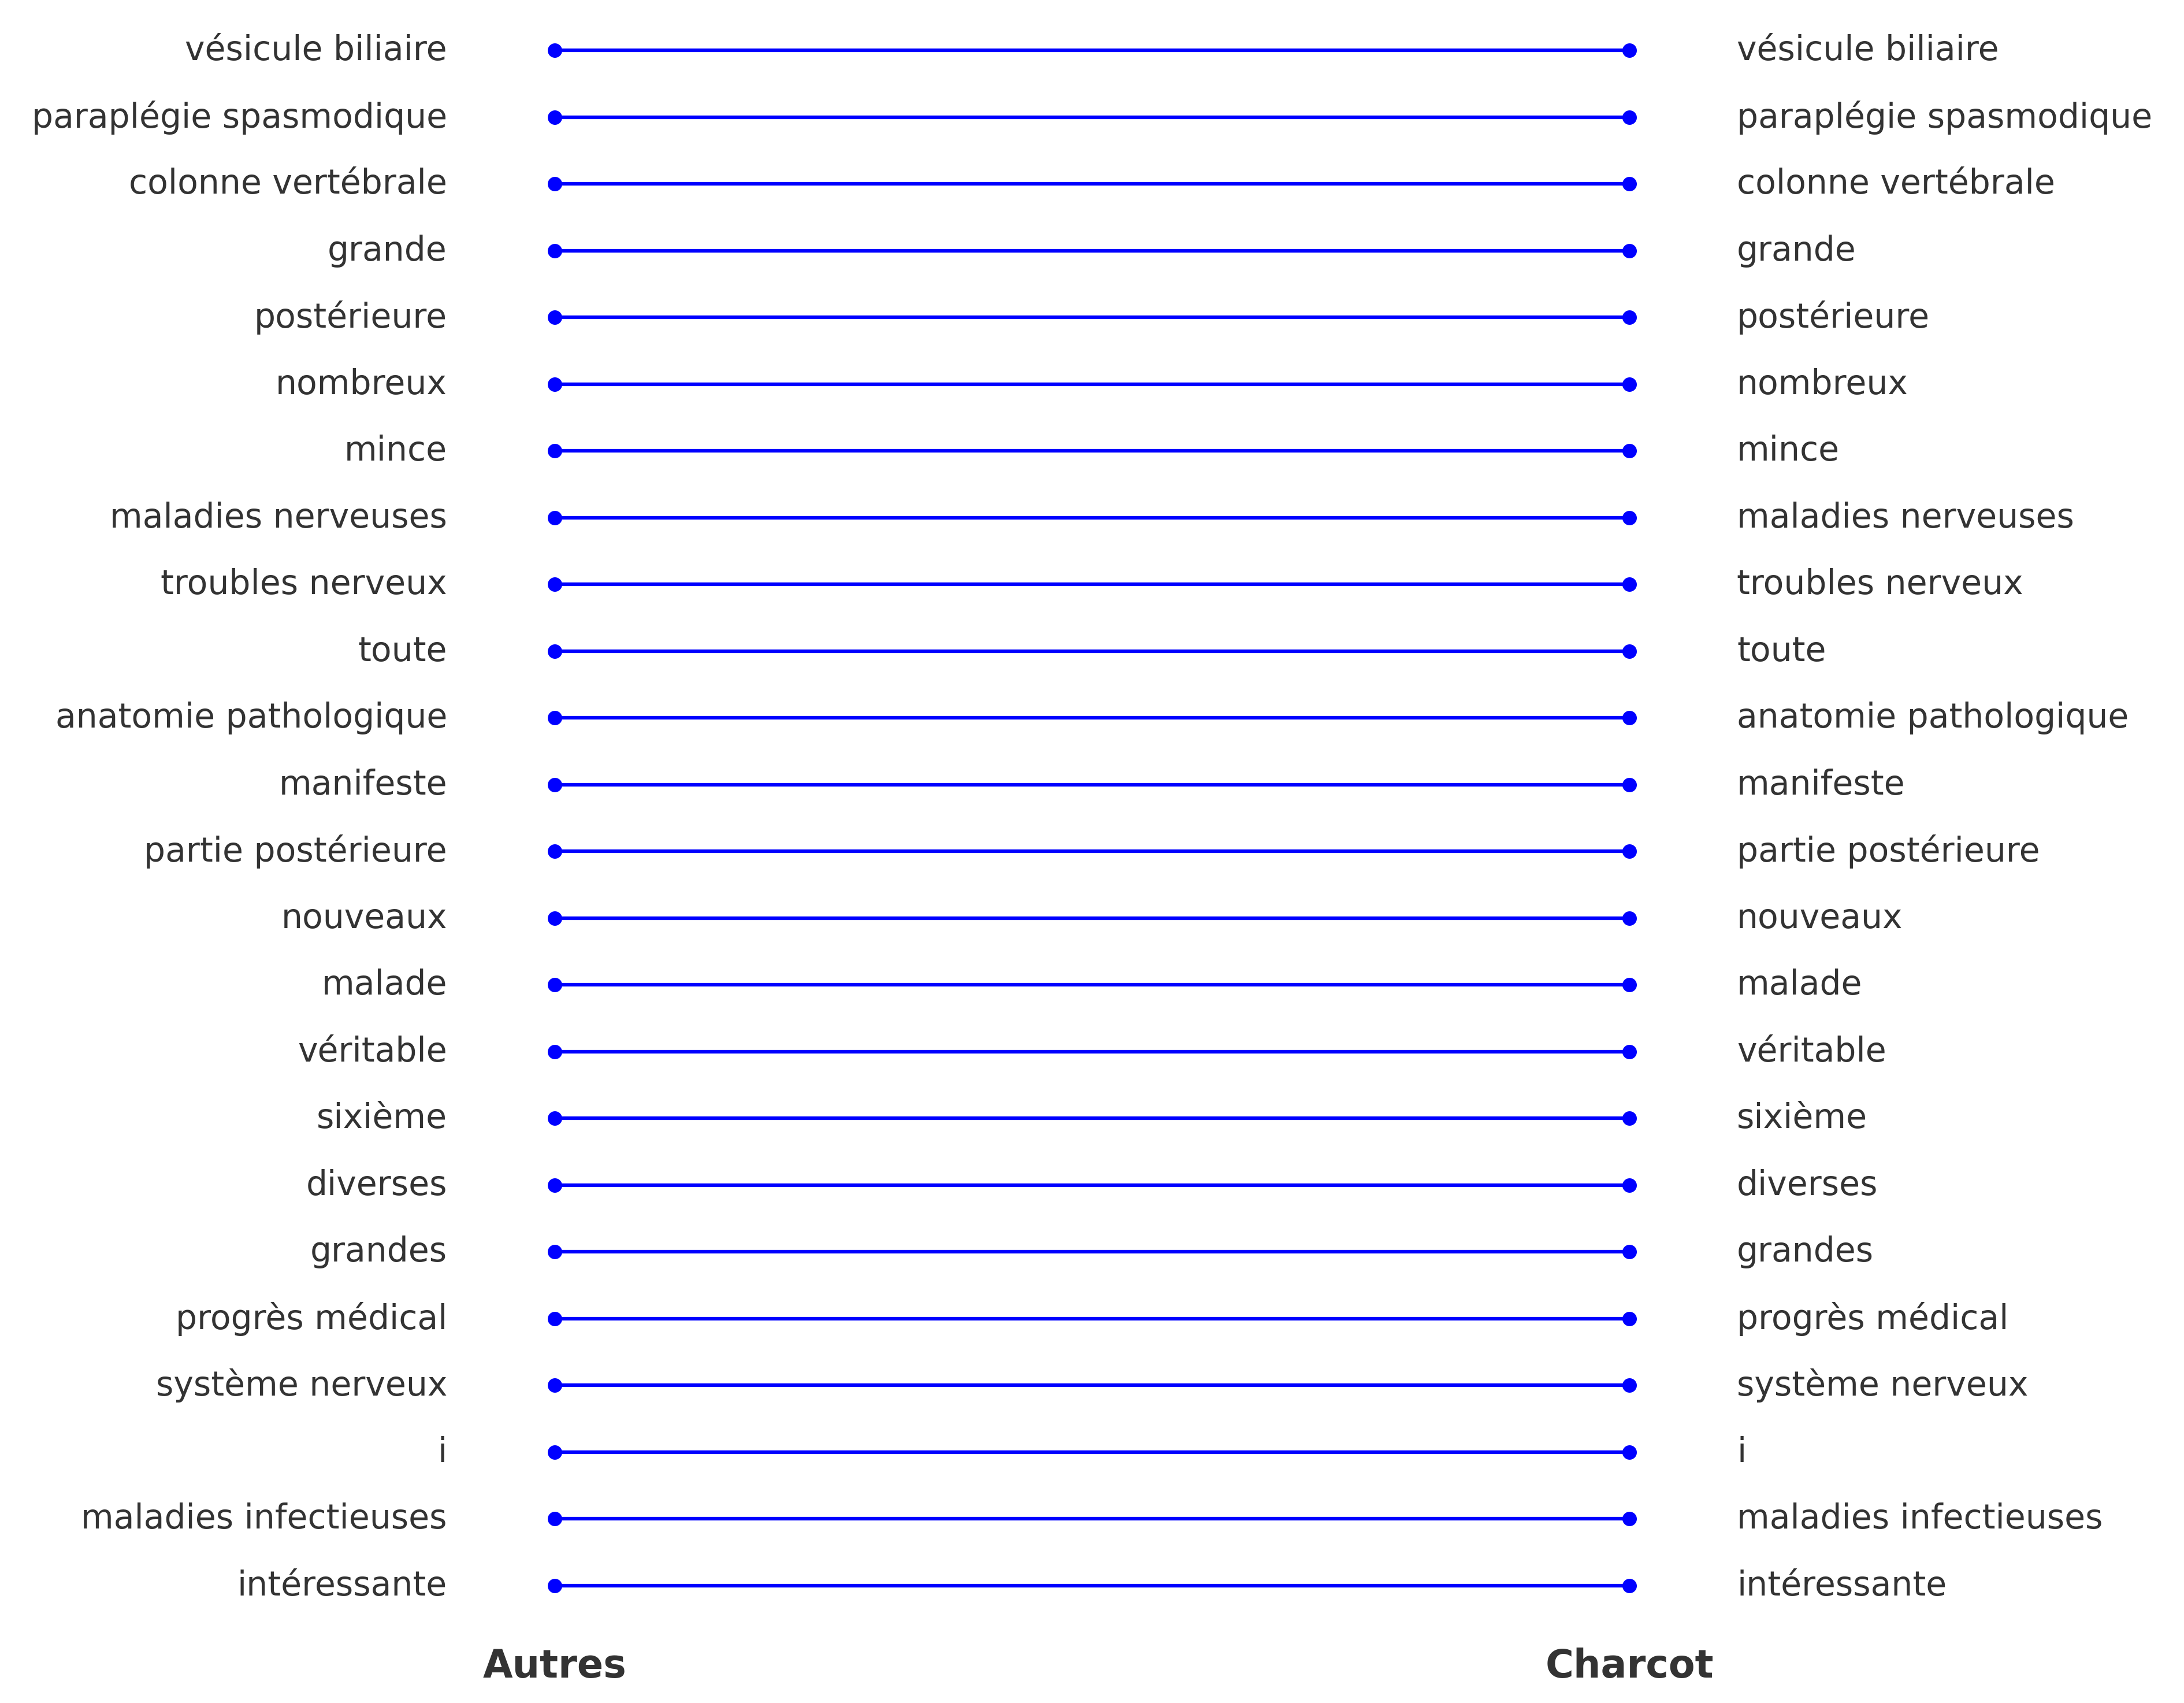
\includegraphics[width=85mm,scale=0.5]{pic/visualisation_termes_dupliques.png}
%        \caption{Les termes communs aux deux corpus selon \texttt{keyphrase-vectorizers}.}
%        \label{fig:enter-label}
%    \end{figure}
%\end{frame}

%\begin{frame}{Termes partagés | \texttt{keyphrase-vectorizers}}
%    \begin{figure}[!ht]
%        \centering
%        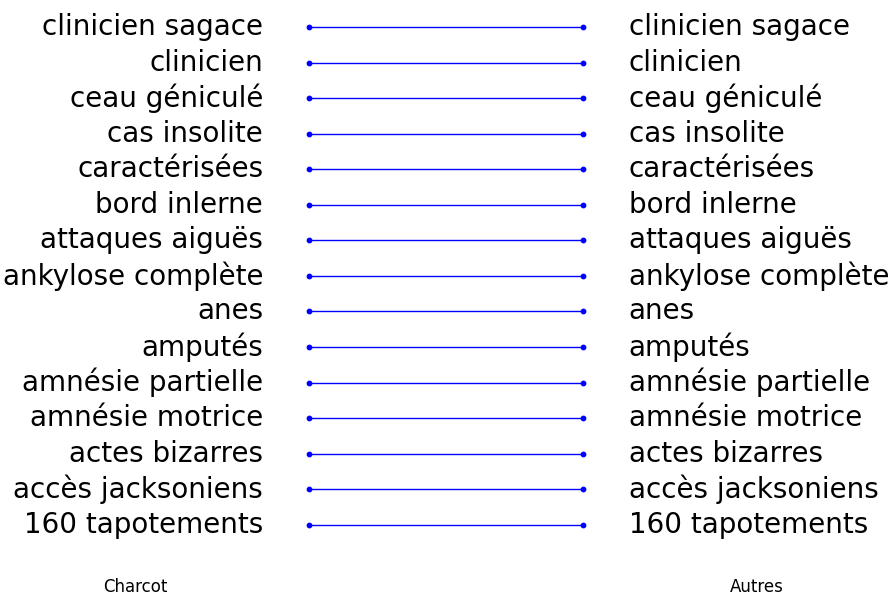
\includegraphics[width=100mm,scale=0.5]{pic/termes_partages_liens.png}
%        \caption{Les termes communs (fréq. = 1) aux deux corpus selon \texttt{keyphrase-vectorizers}.}
%        \label{fig:enter-label}
%    \end{figure}
%\end{frame}

\begin{frame}{Les termes partagés les plus fréquents | \texttt{keyphrase-vectorizers}}
    \begin{figure}[!ht]
        \centering
        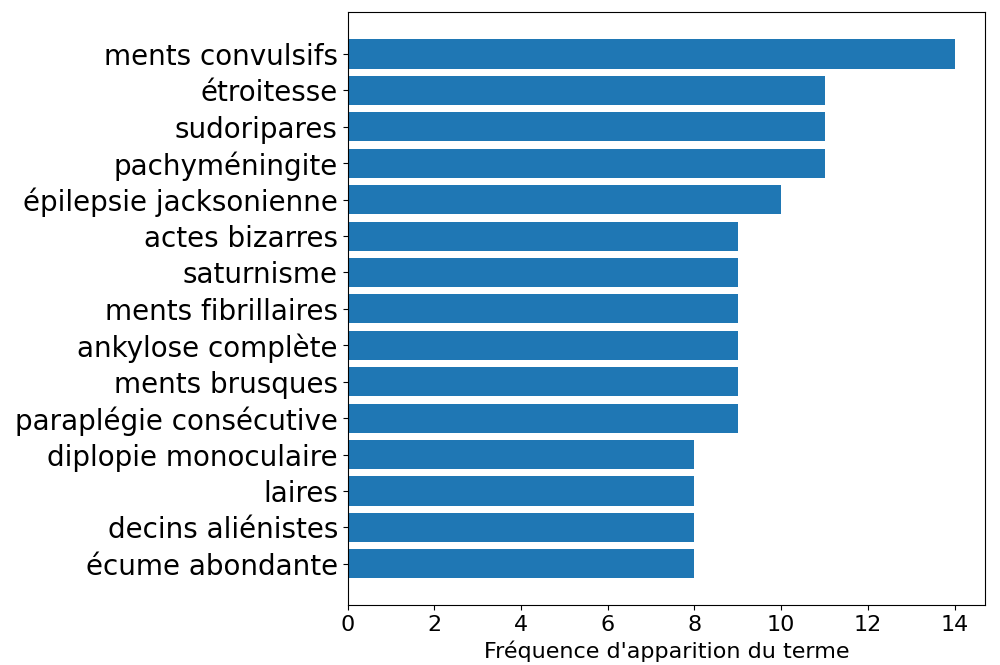
\includegraphics[width=100mm,scale=0.5]{pic/termes_partages.png}
        \caption{Les 15 termes les plus fréquents dans les deux corpus selon \texttt{keyphrase-vectorizers}.}
        \label{fig:enter-label}
    \end{figure}
\end{frame}

\section[Conclusion]{Conclusion}
\begin{frame}{Évolution du projet}
\begin{figure}[h]
    \centering
    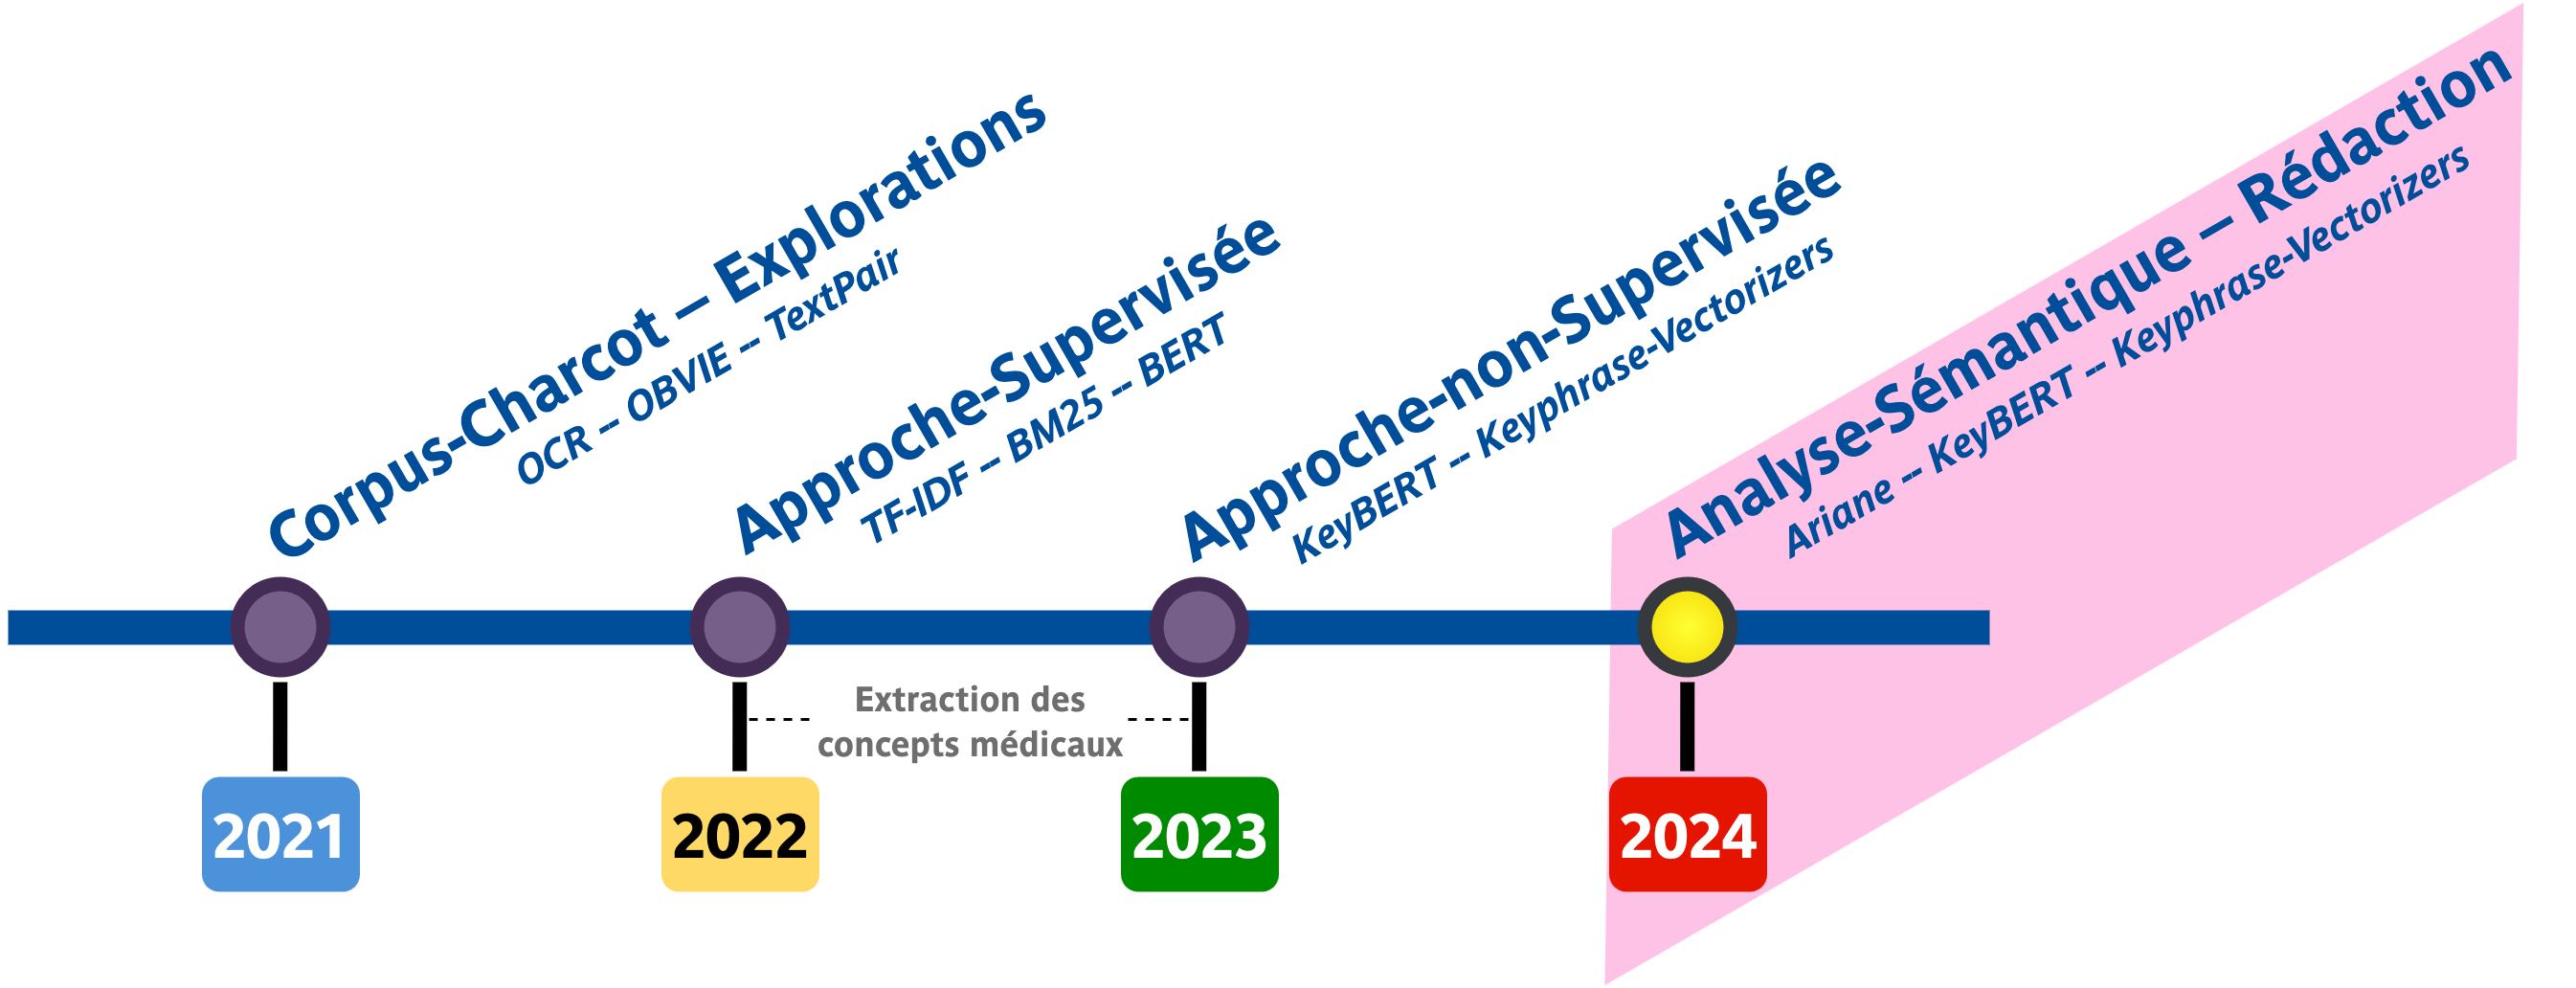
\includegraphics[width=1\textwidth]{pic/timeline_Charcot.png}
    \label{fig:enter-label}
    \caption{Méthodes computationnelles déjà expérimentées et à expérimenter.}
\end{figure}
$\rightarrow$ histoire des concepts {\footnotesize(allem. \textit{Begriffsgeschichte}) \citep{koselleck2011introduction}}
\end{frame}

%\begin{frame}
%\frametitle{Plan}
%    \tableofcontents[sectionstyle=show,subsectionstyle=show/shaded/hide,subsubsectionstyle=show/shaded/hide]
%\end{frame}


%\section[Contexte]{Contexte de recherche}
%\input{1-1_rupture}
%\input{1-2_evolution_hysterie}
%\input{1-3_napoleon}
%\input{2-1_problematique_objectifs}
%
%\section[Objectif]{Problématique et objectif}
%\input{2-2_jonction}
%\input{2-3_question}
%
%\section[Approche supervisée]{Approche supervisée}
%\input{2_methodo}
%\input{supervise}
%\section[Approche non supervisée]{Approche non supervisée}
%\input{non_supervise}
%\section[Conclusion]{Conclusion et recherches futures}
%\input{conclusion}
%\section[État de l'art]{État de l'art}
%\input{sota}
%\section[\textit{PatternRank}]{\textit{PatternRank}}
%\input{patternrank}



% \appendix

\begin{frame}[allowframebreaks]{Références}
\printbibliography

\end{frame}

\end{document}